\documentclass[times, utf8, diplomski, numeric]{fer}
\usepackage{booktabs}
\usepackage{listings}
\usepackage{color}
\usepackage{pdfpages}



\definecolor{lightgray}{rgb}{.9,.9,.9}
\definecolor{darkgray}{rgb}{.4,.4,.4}
\definecolor{purple}{rgb}{0.65, 0.12, 0.82}

\definecolor{mygreen}{rgb}{0,0.6,0}
\definecolor{mygray}{rgb}{0.5,0.5,0.5}
\definecolor{mymauve}{rgb}{0.58,0,0.82}

\lstset{ %
    backgroundcolor=\color{white}, % choose the background color; you must add \usepackage{color} or \usepackage{xcolor}
    basicstyle=\footnotesize, % the size of the fonts that are used for the code
    breakatwhitespace=false, % sets if automatic breaks should only happen at whitespace
    breaklines=true, % sets automatic line breaking
    captionpos=b, % sets the caption-position to bottom
    commentstyle=\color{mygreen}, % comment style
    deletekeywords={...}, % if you want to delete keywords from the given language
    escapeinside={\%*}{*)}, % if you want to add LaTeX within your code
    extendedchars=true, % lets you use non-ASCII characters; for 8-bits encodings only, does not work with UTF-8
    frame=single, % adds a frame around the code
    keepspaces=true, % keeps spaces in text, useful for keeping indentation of code (possibly needs columns=flexible)
    keywordstyle=\color{blue}, % keyword style
    % language=Octave, % the language of the code
    morekeywords={*,...}, % if you want to add more keywords to the set
    numbers=left, % where to put the line-numbers; possible values are (none, left, right)
    numbersep=5pt, % how far the line-numbers are from the code
    numberstyle=\tiny\color{mygray}, % the style that is used for the line-numbers
    rulecolor=\color{black}, % if not set, the frame-color may be changed on line-breaks within not-black text (e.g. comments (green here))
    showspaces=false, % show spaces everywhere adding particular underscores; it overrides 'showstringspaces'
    showstringspaces=false, % underline spaces within strings only
    showtabs=false, % show tabs within strings adding particular underscores
    stepnumber=1, % the step between two line-numbers. If it's 1, each line will be numbered
    stringstyle=\color{mymauve}, % string literal style
    tabsize=2, % sets default tabsize to 2 spaces
    title=\lstname % show the filename of files included with \lstinputlisting; also try caption instead of title
}
%END of listing package%
 
%define JavaScript language
\lstdefinelanguage{JavaScript}{
    keywords=[1]{typeof, new, true, false, function, null, undefined, var, in, of, let, const, class, extends, implements, constructor, super, this, async},
    keywordstyle=[1]\color{blue}\bfseries,  % blue % black
    keywords=[2]{import, from, as, export, default, return, if, for, switch, while, do, else, case, break, continue, await, try, catch, throw},
    keywordstyle=[2]\color{purple}\bfseries,  % purple % black
    keywords=[3]{console, date, number, string, boolean, never, object, error, module},
    keywordstyle=[3]\color{mymauve},
    identifierstyle=\color{black},
    sensitive=false,
    comment=[l]{//},
    morecomment=[s]{/*}{*/},
    commentstyle=\color{mygreen}\ttfamily,  % green % mygray
    stringstyle=\color{red}\ttfamily,  % red % darkgray
    morestring=[b]',
    morestring=[b]",
    morestring=[b]`,
}

%define TypeScript language
\lstdefinelanguage{TypeScript}{
    keywords=[1]{typeof, new, true, false, function, null, undefined, var, in, of, let, const, class, extends, implements, constructor, super, this, async, interface, type, declare, module},
    keywordstyle=[1]\color{blue}\bfseries,  % blue % black
    keywords=[2]{import, from, as, export, default, return, if, for, switch, while, do, else, case, break, continue, await, try, catch, throw},
    keywordstyle=[2]\color{purple}\bfseries,  % purple % black
    keywords=[3]{console, date, number, string, boolean, never, object, error},
    keywordstyle=[3]\color{mymauve},
    identifierstyle=\color{black},
    sensitive=false,
    comment=[l]{//},
    morecomment=[s]{/*}{*/},
    commentstyle=\color{mygreen}\ttfamily,  % green % mygray
    stringstyle=\color{red}\ttfamily,  % red % darkgray
    morestring=[b]',
    morestring=[b]",
    morestring=[b]`,
}
 
\lstset{
    language=JavaScript,
    extendedchars=true,
    basicstyle=\footnotesize\ttfamily,
    showstringspaces=false,
    showspaces=false,
    numbers=left,
    numberstyle=\footnotesize,
    numbersep=9pt,
    tabsize=2,
    breaklines=true,
    showtabs=false,
    captionpos=b
}

\renewcommand{\lstlistingname}{Isječak koda}
\renewcommand{\lstlistlistingname}{Popis isječaka koda}

\newcommand{\razmakp}{\vspace{18pt}}
\newcommand{\razmaks}{\vspace{10pt}}
\newcommand{\uvlakas}{\hspace{0.5cm}}



\begin{document}

\thesisnumber{1937}

\title{Sustav za podršku učenju koncepata deklarativne programske paradigme}

\author{Petar Kovačević}

\maketitle

% Ispis stranice s napomenom o umetanju izvornika rada. Uklonite naredbu \izvornik ako želite izbaciti tu stranicu.
\includepdf{zadatak.pdf}

% Dodavanje zahvale ili prazne stranice. Ako ne želite dodati zahvalu, naredbu ostavite radi prazne stranice.
\zahvala{}

\tableofcontents



% Uvod
\chapter{Uvod}

TODO



% Tehnologije
\chapter{Tehnologije}


% Jezik
\section{Jezik}

Programski jezici implementacije sustava su JavaScript za poslužiteljsku stranu \engl{sever-side} i TypeScript za aplikacijsku, odnosno klijentsku stranu \engl{client-side}.
Na klijentskoj strani je u velikoj mjeri prisutna JSX, odnosno TSX sintaksa.


\razmaks
% JavaScript (ECMAScript)
\subsection{JavaScript (ECMAScript)}

JavaScript je viši programski jezik opće namjene koji se primarno izvodi u internet preglednicima, odnosno uz HTML i CSS (koji nisu jezici opće namjene) jedini je programski jezik kojeg preglednici nativno (bez dodataka) podržavaju.
Sintaksa jezika je slična ostalim jezicima takozvane C obitelji jezika, ali za razliku od njih riječ je o dinamičko-tipiziranom \engl{dynamicly typed} interpretabilnom jeziku.\citep{mdn_js}

Jezik podržava više paradigmi, ali je primarno objektno orijentiran i to, za razliku od drugih popularnih jezika te skupine, baziran na prototipovima \engl{prototype-based}, a ne na razredima.
Ključna razlika između ta dva pristupa je u implementaciji nasljeđivanja. U JavaScript-u se nasljeđivanje odvija proširivanjem \emph{prototipova} koji su posebni tipovi objekata pomoću kojih se stvaraju objekti.\citep{wiki_proto_prog}
Budući da je koncept prototipova većini programera stran i da, zbog dinamičnih tipova u JavaScriptu, neoprezno korištenje može dovesti do nepredviđenih grešaka, od verzije ECMAScript 2015\footnote{
    također poznata pod nazivom ECMAScript 6, skraćeno ES6
} dodani su razredi kao sintaksni šećer \engl{syntax sugar} koje programeri mogu koristiti slično drugim objektno orijentiranim jezicima, a transpilatori\footnote{
    kompilatori, odnosno jezični prevoditelji koji prevode novije verzije JavaScript jezika u starije kako bi stariji preglednici mogli izvršavati napisan kod, primjer: Babel (\url{https://babeljs.io})
} ih prevode u prototipove\citep{mdn_class}.

\razmakp

ECMAScript je pojam koji se često koristi kao alternativno ime za jezik JavaScript, posebice kada se želi naglasiti korištenje modernih novijih verzija jezika.
ECMAScript je ustvari specifikacija skriptnog jezika pod kodovima ECMA-262 i ISO/IEC 16262 kojeg održava međunarodna organizacija Ecma International\footnote{\url{https://www.ecma-international.org}}.
Taj standard implementira više programskih jezika, ali je daleko najpoznatiji JavaScript za kojeg je primarno standard i napisan.
U trenutku pisanja ovog rada najnovija verzija standarda je verzija 9, odnosno ECMAScript 2018.\citep{wiki_es}

\razmaks
% Asinkronost i Promise objekt
\subsubsection{Asinkronost i \emph{Promise} objekt} \label{sec:async}

Ključan detalj za JavaScript i jezike koje se prevode u JavaScript je da se izvode u jednodretvenom okruženju i da je konkurentnost tog okruženja bazirana na modelu petlje događaja \engl{event loop}.
Pojednostavljena verzija tog modela je da za svaki asinkroni događaj (primjerice dohvat podataka s poslužitelja) postoji funkcija povratnog poziva \engl{callback function} i ta funkcija se stavlja u red poruka \engl{message queue}.
Dretva u kojem se izvršava JavaScript kod je ostvarena kao neblokirajuća beskonačna petlja koja, u trenutku kada ne izvršava neki dio koda, provjerava red poruka.
Ako je asinkron događaj elementa izvađenog iz reda gotov, petlja izvršava funkciju povratnog poziva, inače stavlja događaj nazad u red i provjerava idući element reda.\citep{mdn_event_loop}

\razmakp

U praksi se pokazalo da aplikacijska logika često zahtijeva da se neki asinkron događaj poziva nakon drugog asinkronog događaja, odnosno unutar funkcije povratnog poziva prvog događaja bi se pozivao događaj sa svojom funkcijom povratnog poziva.
Ovakav scenarij se često mogao ponoviti i u toj unutarnjoj funkciji povratnog poziva što bi dovelo do teško održivog i teško čitljivog koda kojeg neki programeri zovu „callback hell“ ili „callback pyramid of doom“.

\razmakp % Primjer ugnježđivanja funkcija povratnog poziva
\begin{lstlisting}[language=JavaScript, caption={Primjer ugnježđivanja funkcija povratnog poziva}, label={lst:callback}]
doSomething(function(result) {
  doSomethingElse(result, function(newResult) {
    doAnotherThing(newResult, function(finalResult) {
      console.log('Got the final result: ' + finalResult);
    }, failureCallback);
  }, failureCallback);
}, failureCallback);
\end{lstlisting}
\razmaks

Rješenje za taj problem je došlo u ECMAScript 2015 uvođenjem \emph{Promise} objekta.
\emph{Promise} je poseban tip objekta koji jer reprezentacija nekog asinkronog događaja, odnosno omotava funkciju povratnog poziva tog asinkronog događaja.
Funkcija je omotana u \emph{obećanje} da će se izvršiti i nad tim objektom može se pozivom metode \emph{then} nizati daljnja \emph{obećanja} asinkronih događaja, odnosno definirati što se izvršava nakon uspješnog ili neuspješnog (metoda \emph{catch}) izvršavanja funkcije povratnog poziva.

\razmakp % Primjer korištenja Promise objekta
\begin{lstlisting}[language=JavaScript, caption={Primjer korištenja \emph{Promise} objekta}, label={lst:promise}]
doSomething()
.then(function(result) {
  return doSomethingElse(result);
})
.then(function(newResult) {
  return doAnotherThing(newResult);
})
.then(function(finalResult) {
  console.log('Got the final result: ' + finalResult);
})
.catch(failureCallback);
\end{lstlisting}
\razmaks

Metode \emph{then} i \emph{catch} su nužne jer \emph{Promise} omotava asinkrone operacije i ne može se izravno iz njega iščitati rezultat operacije jer se u trenutku izvršavanja koda ne zna u kojem je stanju \emph{Promise} objekt.

\begin{figure}[!htb] % Životni ciklus Promise objekta
    \centering
    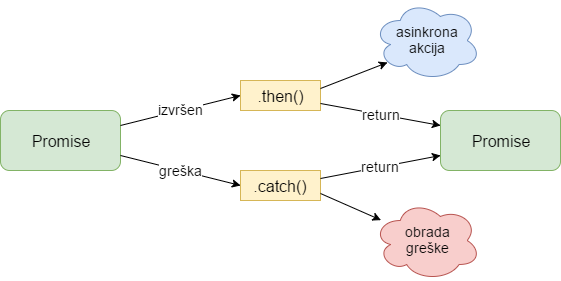
\includegraphics[width=14cm]{images/promise.png}
    \caption{Životni ciklus \emph{Promise} objekta}
    \label{fig:promise_lifecycle}
\end{figure}

\emph{Promise} u svom životnom ciklusu prolazi kroz dva od tri moguća stanja.
Na početku je u pripravnosti \engl{pending} i ovisno o uspješnosti asinkrone operacije odlazi u stanje \emph{ispunjen} \engl{fulfilled} ili \emph{odbijen} \engl{rejected} (vidi sliku \ref{fig:promise_lifecycle}).
U trenutku ulaska u jedno od dva konačna stanja poziva se funkcija ili novi \emph{Promise} definiran kao rezultat funkcije koja je argument \emph{then} ili \emph{catch} metode.
U slučaju da \emph{Promise} uđe u odbijeno stanje, a nema poziva \emph{catch} metode, u aplikaciji će se propagirati greška da odbijeno stanje nije obrađeno \engl{unhandled promise rejection}.\citep{mdn_promise}

\razmakp

Budući da novi koncept \emph{Promise} objekta nije u savršeno pomogao s čitljivošću koda, pogotovo u situacijama kada je nužno obraditi grešku u sredini nekog većeg lanca \emph{Promise} objekata, u specifikaciji ECMAScript 2017 se dodatno uljepšala sintaksa korištenja \emph{Promise} objekata uvođenjem novih ključnih riječi \emph{async} i \emph{await} koji se mogu kombinirati s postojećom \emph{try} i \emph{catch} sintaksom.
Ideja je da se funkcije koje su asinkrone, odnosno vraćaju \emph{Promise} označe ključnom riječi \emph{async}.
Rezultat te funkcije se može odmotati korištenjem ključne riječi \emph{await}.
Time se postiže neblokirajuće čekanje na izvršavanje asinkrone operacije, ekvivalentno tome da se pozvalo \emph{then}\footnote{
    Transpilator u praksi ne prevodi \emph{await} i kod koji slijedi u \emph{then} već prevodi cijelu \emph{async} funkciju u funkciju generator \engl{generator function} gdje samo \emph{await} zamjeni s \emph{yield“} Ta funkcija generator je potom omotana u drugu funkciju koja koristi taj generator da bi iterirala po koracima lanca asinkronih operacija i pozvala \emph{then} za idući dio lanca. Nakon toga je funkcija generator, budući da je i ona relativno novi dodatak (ECMAScript 2015), prevedena u kod koji je u skladu sa starijim standardom.
}.
Za obradu grešaka, umjesto \emph{catch} metode koristi se postojeći \emph{catch} blok.

\razmakp % Primjer korištenja ECMAScript 2017 sintakse
\begin{lstlisting}[language=JavaScript, caption={Primjer korištenja ECMAScript 2017 sintakse}, label={lst:await}]
try {
  const result = await doSomething()
  const newResult = await doSomethingElse(result);
  const finalResult = await doAnotherThing(newResult);
  console.log('Got the final result: ' + finalResult);
} catch (err) {
  failureCallback(err);
}
\end{lstlisting}
\razmaks


\newpage
% TypeScript
\subsection{TypeScript} \label{sec:ts}

TypeScript je programski jezik razvijen od strane tvrtke Microsoft, koji je nadogradnja \engl{superset} nad jezikom JavaScript.
TypeScript proširuje JavaScript sintaksu \footnote{specifično ECMAScript 2015 i kasnije verzije specifikacije sintakse} s tipovima i sučeljima.
Varijable, konstante, funkcije, razredi i elementi razreda mogu se anotirati prikladnim tipovima čija se ispravnost provjerava pri prevođenju TypeScript koda u JavaScript.
Tipovi mogu biti primitivi (\emph{number}, \emph{boolean}, \emph{string}, \emph{symbol}\footnote{
    \emph{Symbol} je novi JavaScript tip, uveden u ECMAScript 2015 standardu (\url{https://developer.mozilla.org/en-US/docs/Glossary/symbol})
}, \emph{void}), vrijednosti (npr. \emph{null}, \emph{undefined}, \emph{'1'}, \emph{1}, \emph{true}…), objekti (\emph{object}), ugrađeni objekti (npr. \emph{Array}, \emph{Date}, \emph{Function}…), posebni TypeScript tipovi (\emph{any}, \emph{never} i \emph{unknown} \footnote{
    \emph{unknown} je uveden tek u TypeScript verziji 3 kao sigurnija alternativa tipu \emph{any}\citep{ts_hand}
}) ili kombinacije spomenutih tipova ostvarenih pomoću sučelja \engl{interface}, unija, presjeka ili kondicionalnih tipova.\citep{gh_ts_spec}\citep{ts_hand}

Korištenje tipova postiže čitljivi i lakše održiv kod,a tipovi omogućavaju se detektiranje nekih čestih JavaScript grešaka pri prevođenju TypeScript koda u JavaScript\footnote{
    Na JSConf Hawaii konferenciji u veljači 2019 godine je predstavnica tvrtke AirBnB izjavila kako su postmortem analizom svojeg dnevnika grešaka i njihovih ispravaka zaključili da bi migriranje iz JavaScript-a u TypeScript eliminirali 38\% grešaka prije nego što se dese, odnosno pri prevođenju u JavaScript\citep{yt_ts}
}.
U isječku koda \ref{lst:typescript} prikazano je nekoliko primjera definiranja i korištenja TypeScript tipova\footnote{
    Napomena: u trenutku pisanja ovog rada najnovija verzija jezika TypeScript je 3.4, no napisani primjeri vrijede i za verziju 2
}.

\razmakp % Primjer definiranja i korištenja TypeScript tipova
\begin{lstlisting}[language=TypeScript, caption={Primjer definiranja i korištenja TypeScript tipova}, label={lst:typescript}]
type Tuple<T> = [T, T];
type NumTuple = Tuple<number>;

function fail(message: string): never {
  throw new Error(message);
}

type GetNameFunction =
  (first: string, last: string, mid?: string) => string;

const getName: GetNameFunction = (first, last, mid?) => {
  if (!first || !last) {
    return fail('First and last name are required');
  }
  if (mid === undefined) {
    return `${first} ${last}`;
  }
  return `${first} ${mid[0]}. ${last}`;
}

interface IPerson {
  name: string;
  age: number;
  doesNameMatch(first: string, last: string): boolean;
}

function areTheSameAge(p1: IPerson, p2: IPerson): boolean {
  return p1.age === p2.age;
}

class Person implements IPerson {
  name: string;
  age: number;
  birthDate: Date;

  constructor(name: string, birthDate: Date) {
    this.name = name;
    this.birthDate = birthDate;
  
    const t: Date = new Date();
    this.age = t.getFullYear() - birthDate.getFullYear();

    const [tMonth, tDate]: NumTuple = [t.getMonth(), t.getDate()];
    const mDiff: number = tMonth - birthDate.getMonth();
    if (mDiff < 0 || (mDiff === 0 && tDate < birthDate.getDate())) {
      this.age--;
    }
  }

  doesNameMatch(first: string, last: string): boolean {
    const otherName = getName(first, last);
    return this.name === otherName;
  }
}

\end{lstlisting}
\razmaks

Bitno je napomenuti da korištenje TypeScript jezika ne isključuje mogućnost korištenja čistog JavaScript koda.
Budući da je TypeScript samo nadogradnja na JavaScript, TypeScript datoteke mogu bez ikakvog problema uvoziti \engl{import} JavaScript datoteke i obratno.
Prevoditelj će u takvoj situaciji samo tretirati sve tipove unutar JavaScript datoteke kao tip \emph{any} koji može označavati bilo koji tip, osim ako prevoditelj ima pristup deklaracijskim datotekama \engl{declaration files} za funkcije i varijable koje se izvoze \engl{export} i koriste unutar JavaScript datoteke.
Deklaracijske datoteke su poseban tip TypeScript datoteka\footnote{označavaju se ekstenzijom „.d.ts“} u kojima se nalazi isključivo deklaracije tipova funkcija i objekata koje se koriste u nekoj JavaScript datoteci ili paketu.\citep{ts_hand}
Budući da su većina paketa koje se koriste u razviju TypeScript projekata napisani isključivo u JavaScript kodu, deklaracijske datoteke često se koriste kako bi se opisalo metode tog paketa i održala sigurnost tipova pri prevođenju jezika.
U nastavku slijedi primjer definicije deklaracijske datoteke za neki paket koji nema vlastitu deklaracijsku datoteku.

\razmakp % Primjer deklaracijske datoteke
\begin{lstlisting}[language=TypeScript, caption={Primjer deklaracijske datoteke}, label={lst:declaration_file}]
import 'my-module';

declare module 'my-module' {
  export function myTestFunction(test: string): boolean;
}
\end{lstlisting}
\razmaks


% JSX i TSX
\subsection{JSX i TSX}

JSX je kratica za JavaScript XML i to je sintaksno proširenje jezika JavaScript gdje se posebne JavaScript funkcije i razredi mogu koristiti kao XML elementi čija struktura nalikuje HTML-u\citep{jsx_spec}.
Korištenje funkcije ili razreda na taj način označava poziv te funkcije, odnosno poziv posebne metode razreda. Sintaksu primarno koristi biblioteka React i paketi koji ovise o toj biblioteci kako bi što čitljivije definirali vizualne komponente koje će se prevesti u HTML kod\citep{react_docs}.
Datoteke koje koriste sintaksu uglavnom završavaju ekstenzijom \emph{.jsx}, odnosno \emph{.tsx} za TypeScript\citep{ts_hand}.
Sav napisani XML kod je ustvari JavaScript, uključivo s elementima koji se zovu isto kao standardni HTML elementi (npr. \emph{div}, \emph{span}, \emph{table}…)\footnote{
    U slučaju tih HTML elemenata riječ je o funkcijama ugrađenih u biblioteku koje su implementirane tako da se pri pozivu i prevođenju povratne vrijednosti u HTML prikažu kao ti isti HTML tagovi.
}tako da pisanje ekstenzije nije nužno osim ako prevoditelj sintakse nije podešen tako da to zahtijeva.


\newpage
% Upravljanje paketima
\section{Upravljanje paketima}

\razmaks
% NPM
\subsection{NPM}

Upravitelj i registar paketa NPM je originalno zamišljen kao upravitelj paketa za izvršno okruženje \emph{Node.js}, no postupno je postao glavni repozitorij za sve JavaScript i TypeScript pakete i najveći repozitorij po broju paketa općenito\citep{med_npm_stats}.
Registar paketa i programsku podršku održava tvrtka Npm, Inc.
U trenutku pisanja ovog rada zadnja stabilna verzija programske podrške za NPM je verzija 6.9\citep{wiki_npm}.

\razmakp

Projekti koji se oslanjaju na NPM za upravljanje paketima moraju sadržavati datoteku \emph{packakge.json} koja se najčešće nalazi u korijenskom direktoriju projekta.
Datoteka može sadržavati neke osnovne informacije o projektu kao što su ime, autor, opis i licenca i neke konfiguracijske detalje, no ključan dio je objekt \emph{dependencies} koji je mapa čiji su ključevi imena paketa koje projekt koristi, a vrijednosti verzije tih paketa\footnote{
    Neki projekti uz \emph{dependencies} imaju i \emph{devDependencies} objekt u kojem se navode paketi koji su nužni isključivo za razvoj, ali ne i za ispravan rad produkcijske verzije projekta. Primjer toga su paketi s deklaracijama TypeScript tipova i ESLint što je linter – dodatak koji provjerava konzistentnost stila pisanja JavaScript koda i upozorava na loše prakse.
}.

Instalacija paketa se odvija tako da se u naredbenoj liniji pozove naredba \emph{npm install} koja potom sve pakete koji su navedeni u \emph{dependencies} i one pakete koje se nalaze u \emph{dependencies} tih paketa i tako rekurzivno preuzima iz NPM repozitorija u mapu \emph{node\_modules}\citep{npm_docs}.
Svi paketi, i oni navedeni u \emph{dependencies} i oni o kojima ti paketi ovise, na istoj razini hijerarhije u mapi \emph{node\_modules}, odnosno svi paketi su u korijenu te mape\footnote{Prije NPM verzije 3 su bili hijerarhijski raspoređeni s obzirom na ovisnosti}.
Razlog tome je ušteda memorije i brža instalacija paketa u slučaju da velik broj paketa dijeli istu ovisnost.
Problem može nastati u slučaju da dva paketa ovise o istom paketu koji su međusobno nekompatibilni.
Ako su pravilno verzionirani, odnosno ako se razlikuju u \emph{Major} verziji\footnote{vidi poglavlje \ref{sec:semver}}, ona verzija paketa koja je kasnije dodana će se instalirati unutar mape paketa koji koristi tu verziju kako ne bi utjecala na rad paketa koji koristi drukčiju verziju\citep{npm_npm3}.


\newpage
% Semantičko verzioniranje
\subsection{Semantičko verzioniranje} \label{sec:semver}

NPM paketi se oslanjaju na to da ih njihovi autori verzioniraju poštujući pravila semantičkog verzioniranja.
Semantičko verzioniranje je način zapisivanja verzija programske podrške gdje se verzija sastoji od tri broja odvojenih točkama.
Prvi broj verzije zove se \emph{Major} i on ukazuje na to da je riječ o potpuno drugačijoj verziji paketa koja nije kompatibilna s verzijama koje se razlikuju u tom broju \engl{breaking change}.
Drugi broj je \emph{Minor} i on ukazuje na to da su se desile promjene u funkcionalnosti i/ili sučelju paketa, ali je verzija kompatibilna sa svim nižim verzijama koji imaju isti \emph{Major} broj \engl{backwards compatible}, odnosno u slučaju da se koristi novija \emph{Minor} verzija od predviđene funkcionirat će jednako.
Treći broj je \emph{Patch} i ukazuje na to da se nije utjecalo na funkcionalnosti i sučelje paketa, već se samo ispravilo greške u implementaciji funkcionalnosti na toj \emph{Major.Minor} verziji\citep{semver}.

\razmakp

NPM pri instalaciji paketa iz naredbene linije, ako mu nije drukčije navedeno pored verzije dodaje znak „\string^“ koji označava da će pri preuzimanju paketa iz repozitorija uzeti najnoviju \emph{Minor} verziju za taj \emph{Major}.
Točnije, u slučaju da je verzija paketa navedena kao „\string^1.2.3“ to znači skini mi bilo koju verziju koja je veća ili jednaka verziji „1.2.3“ i manja od verzije „2.0.0“.
U slučaju da se želi precizirati točnu verziju oznaka se može maknuti ili, ako se želi isključivo skinuti najnoviju \emph{Patch} verziju staviti znak tilda („\string~“)\footnote{
    Upozorenje: Tilda („\string~“) ustvari znači da zadnji navedeni broj može biti veći od onog koji piše. Ako se verzija navede s izostavljenim \emph{Patch} brojem to onda znači da \emph{Minor} može biti veći, odnosno u slučaju da je navedena verzija „\string~1.2“ to znači da u obzir dolazi svaka verzija veća ili jednaka „1.2.0“ i manja od „2.0.0“
}.
Stvari se drukčije ponašaju u slučaju da je \emph{Major} verzija 0, što je karakteristično za pakete koji su još uvijek u ranoj fazi razvoja i nestabilni.
Tada se drugi broj tretira kao da je \emph{Major}, jer on označava da su se desile promjene nekompatibilne s prijašnjom verzijom\citep{npm_docs}.


\newpage
% Poslužiteljska strana
\section{Poslužiteljska strana}

Poslužitelj se pokreće i izvodi u \emph{Node.js} izvršnom okruženju \engl{runtime}, a izgrađen je pomoću radnog okvira \engl{framework} Express.
Podaci se spremaju u MongoDB dokument bazu podataka \engl{document-based database} kojoj se pristupa koristeći biblioteku Mongoose (koja se ujedno koristi i za modeliranje podataka).


\razmaks
% Node.js
\subsection{Node.js}

\emph{Node.js} (u daljnjem tekstu Node) je izvršno okruženje za JavaScript izgrađeno nad Chrome V8 mehanizmom \engl{engine}.
Node je primarno namijenjen izgradnji skripti za web poslužitelje i alate naredbene linije \engl{command line tools}.
Ključna prednost koju nudi u izgradnji web poslužitelja je što omogućava da se koristi isti jezik (JavaScript ili jezik koji se prevodi u JavaScript) koristi za izgradnju poslužiteljske i klijentske strane, što olakšava razvoj u slučaju kada isti razvojni tim programira i poslužiteljsku i klijentsku aplikaciju\citep{wiki_node}.

Druga prednost je u konkurentnom model jezika JavaScript \footnote{vidi poglavlje \ref{sec:async}} koji omogućava i potiče neblokirajuće, odnosno asinkrone ulazno-izlazne operacije \engl{asynchronous I/O}, što pomaže u izgradnji skalabilnih i brzih web poslužitelja.
Naravno taj isti model onemogućava stvaranje zasebnih dretvi u jednom Node procesu. Node proces pri pokretanju stvara fiksan broj dretvi koje su potrebne za njegov rad i ne nudi programeru stabilno sučelje za stvaranje novih dretvi.
Od verzije 10.5 uveden je eksperimentalan modul \emph{worker-threads}\footnote{
    korištenje modula mora se eksplicitno navesti pri pokretanju Node procesa sa zastavicom \emph{-{}-experimental-worker}
} koji omogućava stvaranje novih dretvi kako bi se sinkrone operacije zahtjevne za procesor \engl{CPU intensive} mogle prebaciti na njih.
Način na koji se ovaj problem rješavao do sada je bio stvaranje novih procesa pomoću postojećeg Node sučelja ili vanjskih paketa\citep{art_node}.

Svaka parna verzija ima podršku za održavanje \engl{long termn support} koja počinje kada krene razvoj sljedeće neparne verzije.
U trenutku pisanja ovog rada verzija 10 ima tu podršku, a uskoro kreće podrška za verziju 12\footnote{od 10. listopada 2019.}\citep{wiki_node}.


\newpage
% Express
\subsection{Express}

Express (poznat još i kao \emph{Express.js}) je minimalistički radni okvir \engl{framework} koji nadograđuje Node sučelje i module za gradnju web poslužitelja s naprednim mogućnostima usmjeravanja \engl{routing} i opcionalnim korištenjem mehanizama predložaka \engl{template engines} za izgradnju web stranica.
Napredne mogućnosti usmjeravanja olakšavaju razdvajanje koda s obzirom na korijenske API rute (korijenske resurse REST arhitekturnog stila), dodavanje međusloja sloja \engl{middleware} u cjevovod \engl{pipeline} specifičnih ruta, serviranje statičkih datoteka i konfiguriranje privremene memorije \engl{cache}.

U trenutku pisanja ovog rada najnovija verzija radnog okvira je verzija 4 i radi u svim verzijama Node okruženja iznad verzije 0.10\citep{gh_express}.


\razmaks
% MongoDB
\subsection{MongoDB} \label{sec:mongo}

\emph{MongoDB} (u daljnjem tekstu Mongo) je NoSQL sustav baza podataka, specifično riječ je o dokument sustavu baza podataka gdje su dokumenti predstavljeni u JSON\footnote{
    \emph{JavaScript Object Notation} – način reprezentacije podataka kao JavaScript objekata - \url{https://www.json.org}
} formatu.
Dokumenti nisu zapravo spremljeni u JSON, već u BSON (\emph{binary JSON}) formatu, što je binarna serijalizacija proširenih JSON objekata koje Mongo koristi za spremanje podataka i upita.
Prošireni JSON znači da Mongo podržava neke tipove koji ne postoje u standardnom JSON-u i JavaScript-u kao što su cjelobrojni brojevi (\emph{int} i \emph{long}), precizni 128 bitni brojevi (\emph{decimal}), binarni podaci i poseban tip za primarne ključeve dokumenata.

Mongo dokumenti su posloženi u kolekcije \engl{collections}.
Kolekcije u praksi predstavljaju dokumente sličnog tipa i namijenjene su tome da se nad njima vrše upiti.
Upiti u Mongo interaktivnom okruženju ostvaruju se u JavaScript jeziku pozivom prikladne funkcije nad kolekcijom (npr. \emph{find}) i predavanjem JavaScript/JSON objekata kao argumente funkcije za izgradnju upita. Upiti su atomarni \engl{atomic} nad pojedinim dokumentom, no od Mongo verzije 4 postoji transakcijski API pomoću kojeg je moguće ostvariti atomarnost na razini sjednice \engl{session}\footnote{
    funkcionalnost transakcija relativno je nova i još uvijek u beta fazi razvoja za distribuirane Mongo sustave
}\citep{mongo}.

Budući da je riječ o NoSQL bazi podataka, ne postoje relacije, odnosno automatski održavane poveznice između dokumenta.
Za većinu aplikacija ovo nije problem jer princip kojim se modeliraju dokumenti u kolekciji nije isti kao modeliranje zapisa u relacijskoj bazi.
Mongo dokumenti modeliraju se kao agregati podataka, odnosno dokumenti koji su u izravnoj ovisnosti o drugom dokumentu nalaze se unutar tog dokumenta.
Tipičan primjer toga je račun nakon kupovine i stavke na tom računu.
Gdje bi u relacijskom sustavu to bile dvije tablice, u Mongo sustavu se ta situacija modelira na način da su stavke računa lista objekata koja se nalazi unutar dokumenta račun.
Na ovaj način jednostavno se može izgraditi distribuiran sustav baze podataka jer je svaki dokument ustvari agregat neovisan o drugim dokumentima.
Naravno u praksi poveznice između dokumenata su nekad nužne i tada se za njihovo održavanje treba brinuti unutar aplikacijske logike.


\razmaks
% Mongoose ODM
\subsection{Mongoose ODM}

Mongoose je JavaScript ODM (krat. \emph{Object Data Model}) biblioteka koja olakšava korištenje Mongo baze podataka.
ODM biblioteke služe za modeliranje podataka NoSQL baza podataka slično kako ORM (krat. \emph{Object Relational Model}\footnote{
    Pojam je različit od \emph{object-relational mapping} koji označava mapiranje relacijskih podataka u objekte i obratno. Za oba pojma često se koristi ista kratica i većina \emph{object relational model} biblioteka implementira i \emph{object-relational mapping}
}) biblioteke služe za modeliranje relacija u razrede, odnosno objekte. U Mongoose biblioteci podaci se modeliraju pomoću sučelja koji se zove \emph{Schema}.
To sučelje se onda koristi za definiranje \emph{Model} objekta.
\emph{Model} objekt predstavlja Mongo kolekciju, čiji dokumenti nužno odgovaraju obliku kakav je definiran pomoću \emph{Schema} objekta, i služi za pozivanje upita nad kolekcijom i kreiranje instanci modela.
Instanca modela predstavlja jedan specifičan dokument koji odgovara \emph{Schema} definiciji objekta tog istog modela.
Na ovaj način se Mongo dokumenti u aplikaciji mogu proširiti s validacijskim slojem i metodama, odnosno dokumenti postaju objekti koji u sebi sadržavaju dio domenske logike za taj agregat\citep{mongoose}.

Mongoose je implementiran tako da ovisi o i koristi službeni Mongo driver za Node, kojem se može pristupiti iz globalnog Mongoose objekta u slučaju da postoji potreba za nekim naprednim Mongo driver mogućnostima koje Mongoose sučelje ne nudi izravno\footnote{\url{https://docs.mongodb.com/ecosystem/drivers/node}}.
U trenutku pisanja ovog rada najnovija verzija Mongoose paketa je 5.6, a paketi iznad verzije 5.2 (uključivo) zahtijevaju MongoDB Server verzije 4.0 ili iznad.

Primjer korištenja Mongoose biblioteke nalazi se u poglavlju \ref{sec:data} u isječku koda \ref{lst:schema}.


\newpage
% Aplikacijska (klijentska) strana
\section{Aplikacijska (klijentska) strana}

Klijentska aplikacija izrađena je koristeći biblioteku React po predlošku i konfiguraciji paketa Create React App.
Izgled aplikacije je stiliziran primarno koristeći radni okvir \engl{framework} Bootstrap, a elementi radnog okvira korišteni su kao React komponente pomoću React Bootstrap implementacije.
Budući da je React biblioteka za izgradnju jednostraničnih \engl{single page} web aplikacija, za navigaciju po različitim dijelovima aplikacije koristi se paket React Router, dok se stanjem aplikacije upravlja pomoću biblioteke Redux.
STORM React Diagrams biblioteka koristi se za izgradnju dinamičnih dijagrama koji su ključan dio aplikacije, a Axios biblioteka se koristi za komunikaciju s poslužiteljem.


\razmaks
% React
\subsection{React} \label{sec:react}

React je JavaScript biblioteka otvorenog koda namijenjena brzoj i jednostavnoj izgradnji korisničkih sučelja.
Razvijena je od strane Facebooka 2013. godine i zadnja stabilna verzija u trenutku pisanja ovog rada je 16.8.6.\citep{gh_react_changelog}.
U izvorima se biblioteka također može naći pod nazivima „React.js“ i „ReactJS“, dok je „React Native“ radni okvir za razvoj mobilnih aplikacija u jeziku JavaScript na sličan način kako se web aplikacije grade u React-u\citep{wiki_react}.
Iako je React biblioteka \engl{library}, nije u potpunosti netočno zvati je radnim okvirom \engl{framework}.
Tijekom godina nakupilo se mnoštvo biblioteka i radnih okvira za korištenje sa samim React-om, da se pod izrazom React često podrazumijeva i njihovo korištenje, što daje dojam cjelokupnog radnog okvira. No, po svojoj definiciji je biblioteka.

React se koristi za razvoj jednostraničnih \engl{single page} web aplikacija.
Produkcijska verzija React stranice često se sastoji od jedne male HTML datoteke (reda veličine dvadesetak linija koda) i JavaScript datoteke od nekoliko desetaka tisuća linija koda.
Razlog je u tome što je sav sadržaj stranice ugrađen u JavaScript kako bi se mogao dinamički mijenjati.

\razmakp

React koristi virtualni DOM \engl{virtual DOM}.
DOM (krat. \emph{Document Object Model}) je memorijska reprezentacija web stranice, odnosno dokumenta – primarno logičkog stabla HTML elemenata\citep{mdn_dom}.
Virtualni DOM je apstrakcija standardnog HTML DOM-a koja se koristi kako bi se izbjegle skupe operacije dodavanja i brisanja elemenata u DOM-u.
Efikasnim upravljanjem virtualnim DOM-om, elementi se ažuriraju u stvarnom DOM-u samo kada je to potrebno, odnosno ažuriraju se isključivo elementi koji su se promijenili\citep{med_vdom}.
Primjerice, nepotrebno je da se svaki put iznova crta (odnosno iščitava iz HTML dokumenta) navigacija, ako se isključivo mijenja sadržaj ispod nje.

\razmakp
% Komponente
\subsubsection{Komponente}

Filozofija React-a je rastaviti korisničko sučelje na komponente kao ponovno iskoristive izolirane cjeline.
Instance komponenti se, slično HTML DOM elementima, organiziraju u strukturu stabla, no za razliku od HTML DOM elemenata, komponente mogu imati vlastito stanje i logiku. React komponente ostvarene su ili kao funkcije koje vraćaju JSX element i zovu se funkcijske komponente \engl{functional components}, ili kao razredi koji nasljeđuju razred \emph{React.Component} koji se zovu razredne komponente \engl{class components}.
Oba načina implementacije stvaraju objekte koji su tipa \emph{React.Component} i prolaze kroz iste faze životnog ciklusa \engl{lifecycle}, no razredne komponente mogu imati vlastito stanje i imaju pristup metodama koje se pozivaju u različitim fazama životnog ciklusa \engl{lifecycle methods}\citep{react_docs}.
Funkcijske komponente u praksi se koriste za implementaciju jednostavnijih komponenti.

\razmakp % Primjer funkcijske i razredne komponente
\begin{lstlisting}[language=JavaScript, caption={Primjer funkcijske i razredne komponente}, label={lst:component}]
import * as React from 'react';

function HelloWorldAsAFunction() {
  return <h1>Hello World</h1>;
}

class HelloWorldAsAClass extends React.Component {
  render() {
    return <h1>Hello World</h1>;
  }
}
\end{lstlisting}
\razmaks

Struktura stabla komponenti znači da su komponente posložene hijerarhijski, odnosno komponente djeca \engl{child components} su ugniježđene u roditeljskoj komponenti \engl{parent component}.
Svaka komponenta može primiti podatke putem svog \emph{props} objekta od svoje roditeljske komponente\citep{react_docs}.
React projekti često prate obrazac podijele komponenti na \emph{pametne} i \emph{glupe} odnosno komponente koje sadrže logiku (često nazvane \emph{container components} i prezentacijske komponente \engl{presentational components}.
Prezentacijske komponente nemaju vlastito stanje, već samo primaju podatke i akcije putem \emph{props} objekta od svojih roditelja, a sav ostali kod koje sadrže odnosi se isključivo na prezentacijsku logiku, odnosno kako će se komponenta prikazati. Roditeljska \emph{pametna} komponenta implementira vlastito stanje i sve akcije koje se dešavaju u toj komponenti i svim prezentacijskim komponenata koja su joj djeca\citep{med_comp}.

Jednostavan primjer toga je tablica s redcima koji se mogu brisati na klik gumba.
Redak i gumb u retku su prezentacijske komponente, dok je tablica pametna komponenta.
Tablica za stanje ima listu svih redaka i podataka u njima i definira funkciju brisanja retka.
Svakoj komponenti \emph{Redak} komponenta \emph{Tablica} prosljeđuje podatke za taj redak i funkciju koja briše taj redak.
Komponenta \emph{Redak} potom definira prikaz podataka i prosljeđuje komponenti \emph{Gumb} funkciju brisanja.
Komponenta \emph{Gumb} veže primljenu funkciju brisanja na svoj klik događaj \engl{onclick event}.
Primjer opisanog scenarija nalazi se u isječku koda \ref{lst:component_props}.

\razmakp % Primjer prosljeđivanja podataka i akcija iz roditeljske komponente
\begin{lstlisting}[language=JavaScript, caption={Primjer prosljeđivanja podataka i akcija iz roditeljske komponente}, label={lst:component_props}]
import * as React from 'react';

class Tablica extends React.Component {
  constructor(props) {
    super(props);
    this.state = {
      rows: props.rows,
    };
  }

  deleteRow = (rowId) => {
    this.setState((state) => ({
      rows: state.rows.filter((row) => row.id !== rowId)
    }));
  }

  render() {
    return (
      <table>
        {this.state.rows.map((row) => (
          <Redak
            key={row.id}
            data={row.data}
            deleteRow={this.deleteRow.bind(row.id)}
          />
        ))}
      </table>
    );
  }
}

function Readak(props) {
  return (
    <tr key={props.key}>
      <div>{props.data}</div>
      <Button onClick={props.deleteRow} text="Obrisi" />
    </tr>
  );
}

function Button(props) {
  return <button onClick={props.onClick}>{props.text}</button>;
}
\end{lstlisting}
\razmaks

\noindent Svaka komponenta ima tri faze životnog ciklusa:

\begin{enumerate}
    \item Početna faza postavljanja \engl{mount}, koja se događa nakon instanciranja objekta komponente, pri njegovom dodavanju u Virtualni DOM.
    \item Faza promjena \engl{update}, u kojoj je instanca većinu vremena. U ovoj fazi dešava se svako ponovno prikazivanje \engl{rerender} instance komponente, najčešće zbog promjene stanja ili ulaznih parametara (\emph{props}).
    \item Faza rastavljanja \engl{unmount} je završna faza komponente koja se dešava kada se instanca uklanja iz Virtualnog DOM-a
\end{enumerate}

\noindent Poznavanje fazi životnog ciklusa komponente je ključno ne samo za razumijevanje ponašanja React komponenti, već zato što se kompleksna logika unutar komponente ostvaruje proširivanjem metoda razreda \emph{React.Component} koje su direktno vezane uz faze životnog ciklusa.
Elementi razreda \emph{React.Component} i svakog razreda koji ga nasljeđuje su\citep{react_docs}:

\begin{enumerate}[label=(\alph*)]

    \item konstruktor
    
    Standardni konstruktor razreda koji se poziva pri stvaranju nove instance. Konstruktor prima \emph{props} objekt i u njemu se može definirati sva sinkrona logika koja se treba desiti prije faze postavljanja, odnosno pri inicijalizaciji objekta komponente.

    \item svojstva \emph{props} i \emph{state}
    
    Oba svojstva instance komponente su objekti koji se mogu isključivo čitati \engl{read-only}.
    Objekt \emph{props} komponenta dobiva putem svog roditelja, odnosno razreda ili funkcije koji poziva komponentu, i jedino ga roditelj može mijenjati.
    Objekt \emph{state} je opcionalan i predstavlja stanje komponente. Objekt se mijenja isključivo pozivom metode \emph{setState}.

    \item statička svojstva \emph{defaultProps} i \emph{displayName}
    
    Objekt \emph{defaultProps} je svojstvo razreda komponente i definira vrijednosti svojstava objekta \emph{props} u slučaju da nisu zadani \engl{undefined}, dok je \emph{displayName} tekst koji se koristi isključivo za lakše pronalaženje grešaka pri razvoju.

    \item metoda \emph{render}
    
    Ovo je ključna metoda i jedina metoda koju nužno implementira svaka React komponenta. Povratna vrijednost metode je JSX element, odnosno stablo JSX elemenata koje definira prikaz komponente.

    \item metode \emph{setState} i \emph{forceUpdate}
    
    Ove dvije metode su jedine koje se ne mogu proširiti, već isključivo naslijediti od \emph{React.Component}.
    Metoda \emph{forceUpdate}, kako joj i ime govori, forsira komponentu da se ažurira, odnosno ponovno izvodi ciklus faze promjene u kojoj poziva metodu \emph{render}.
    Metoda \emph{setState} je asinkrona metoda koja služi za postavljanje stanja.
    Ona ne vraća \emph{Promise} objekt\footnote{vidi poglavlje \ref{sec:async}}, već prima funkciju povratnog poziva kao svoj drugi argument.
    Razlog ovakve implementacije je optimizacija, odnosno React višestruke pozive metode \emph{setState} koji su se desili u kratkom vremenskom zna spojiti u jedno ažuriranje stanja.
    Ova optimizacija je bitna jer ažuriranje stanja u većini situacija znači ažuriranje cijele komponente (s ponovnim pozivom \emph{render} metode) što je potencijalno skupa operacija.

    \item metode životnog ciklusa: \emph{componentDidMount}, \emph{shouldComponentUpdate},
    \break \emph{getSnapshotBeforeUpdate}, \emph{componentDidUpdate} i \emph{componentWillUnmount}.
    
    Metode se redom pozivaju: neposredno nakon postavljanja komponente, neposredno prije poziva \emph{render} metode, u trenutku izvršavanja \engl{commit} povratne vrijednosti \emph{render} metode na DOM, neposredno ažuriranja komponente, i neposredno prije rastavljanja komponente.
    Metoda \emph{shouldComponentUpdate} može utjecati na životni ciklus na način da ovisno o njenoj povratnoj vrijednosti (koja je logičkog tipa – engl. \emph{boolean} će se ažuriranje komponente, odnosno poziv metode \emph{render}, desiti ili prekinuti.
    Ako komponenta nasljeđuje razred \emph{React.PureComponent}, nema pristup ovoj metodi jer je već implementirana u tom razredu.
    Razred \emph{React.PureComponent} implementira metodu \emph{shouldComponentUpdate} na način da radi plitku usporedbu \engl{shallow compare} svojstava objekata \emph{props} i \emph{state} od trenutnog i budućeg stanja. Ako se neki od svojstava razlikuje (po referenci za objekte, a po vrijednosti za primitivne vrijednosti) ažuriranje će se desiti, u suprotnom stanje komponente se smatra nepromijenjenim. Ovaj način usporedbe je jako brz, stoga se \emph{React.PureComponent} često koristi za optimizaciju performansi\citep{react_docs}.

    \item statička metoda životnog ciklusa \emph{getDerivedStateFromProps}
    
    Ova razredna metoda poziva se prije poziva metode \emph{shouldComponentUpdate} i ima pristup objektima \emph{props} i \emph{state} u tom trenutku

    \item zastarjele metode životnog ciklusa: \emph{UNSAFE\_componentWillMount},
    \break \emph{UNSAFE\_componentWillReceiveProps} i \emph{UNSAFE\_componentWillUpdate}
    
    Ove metode ne moraju nužno biti prefiksirane s \emph{UNSAFE\_} i u prethodnim verzijama React-a (prije verzije 16.3) nemaju taj prefiks.
    Prefiks je dodan kako bi se naglasilo da će metode biti uklonjene u verziji 17 i da ih se preporuča ne koristiti.
    Razlog zašto nisu odmah uklonjene je da bi ljudi lakše migrirali s React verzije 15 na verziju 16\citep{react_16_3}.

    \item metoda \emph{componentDidCatch} i statička metoda \emph{getDerivedStateFromError}
    
    Ovo su metode koje se koriste u svrhu upravljanja greškama \engl{error handling} i dio su skupa novih metoda koje su dodane u React 16\footnote{
        Uz njih su dodane i metode \emph{getSnapshotBeforeUpdate} i \emph{getDerivedStateFromProps}. Ključno je napomenuti da nisu sve metode dodane odmah u verziji 16.0, već postupno u verzijama 16.0, 16.3 i 16.6\citep{gh_react_changelog}.
    }\citep{react_error}.
\end{enumerate}
\razmaks

Na slici TODO prikazan je pojednostavljen dijagram u kojim fazama se pozivaju metode komponente.


\razmaks
% Create React App
\subsection{Create React App} \label{sec:cra}

Paket Create React App je službeni predložak koji apstrahira od programera većinu konfiguracije i paketa koji su nužni za razvoj React aplikacija.
Instalacijom i pokretanjem paketa korisnik dobiva konfiguriran prevoditelj Babel\footnote{\url{https://babeljs.io}} s opcionalnom TypeScript podrškom\footnote{
    Podrška za TypeScript je došla u Babel verziji 7, a u trenutku pisanja ovog rada Babel-ov TypeScript prevoditelj ne podržava sve dijelove TypeScript sintakse. Primjer toga su prostori imena \engl{namespace} i konstantne enumeracije \engl{const enums}\citep{ms_dev_babel}.
}, upravitelj modulima Webpack\footnote{\url{https://webpack.js.org}} s postavljenim serverom za razvoj i skripte za pokretanje i izgradnju aplikacije.
U slučaju da korisnik želi izmijeniti ili proširiti predefinirane postavke, to može jednostavnim pokretanjem skripte \emph{eject} koja izbacuje i otkriva svu konfiguraciju i pakete koji su se nalazili unutar paketa Create React App.
Ova akcija je nepovratna, nakon nje više se ne može jednostavno ažurirati predložak, već se mora ručno ažurirati svaki od paketa i dijelova konfiguracije\citep{gh_cra}.

\razmakp

Za izgradnju aplikacijske strane u ovom radu koristio se predložak koji se dobije naredbom „\emph{create-react-app <ime\_aplikacije> -{}-typescript}“ s Create React App verzijom 3.0.
Početna struktura projekta nakon pokretanja naredbe može se vidjeti na TODO


\razmaks
% React Router
\subsection{React Router}

Činjenica da je web aplikacija jednostranična ne mora začiti da korisnik ne može pristupati različitim dijelovima, odnosno stanjima te aplikacije pomoću poveznica.
Korisnik želi imati mogućnosti da putem poveznice izravno dođe do nekog dijela aplikacije ili da se vrati na prethodno stanje aplikacije klikom \emph{Nazad} u pregledniku, kao što to može s klasičnim web stranicama\footnote{Ovdje se izraz \emph{web stranica} odnosi na engl. \emph{website}, odnosno kolekciju stranica \engl{web page}.}.

Takvo ponašanjem unutar React aplikacije može se postići koristeći bibliteku React Router („\emph{react-router}“), točnije paket \emph{react-router-dom} koji je implementacija React Router API-ja za web, odnosno namijenjena aplikacijama koje se izvršvaju u web pregledniku\footnote{
    Nije potrebno instalirati oba paketa jer paket \emph{react-router-dom} sadrži u sebi \emph{react-router}.
    Paket \emph{react-router} je ustvari bazni paket koji koriste specifične implementacije kao što su \emph{react-router-dom} i \emph{react-router-native} (implementacija namijenjena korištenju u React Native radnom okviru).
}.
Pomoću njega dobije se pristup promjenjivom objektu povijesti \engl{history}, kojim se služi kao s povijesti preglednika, i gotovim navigacijskim komponentama za upravljanje s tom povijesti.
Jedini uvjet za korištenje tih mogućnosti je da su komponente koje ih koriste ugniježđene u komponenti \emph{Router}\citep{react_router}.

\razmakp %
\begin{lstlisting}[language=JavaScript, caption={Primjer korištenja React Router biblioteke}, label={lst:react_router}]
import * as React from 'react';
import {
  BrowserRouter as Router, Route, Link
} from 'react-router-dom';

const Home = () => ( <div> <h2>Home</h2> </div> );
const About = () => ( <div> <h2>About</h2> </div> );

class App extends React.Component {
  render() {
    return (
      <Router>
        <div>
          <ul>
            <li><Link to="/">Home</Link></li>
            <li><Link to="/about">About</Link></li>
          </ul>
          <Route exact path="/" component={Home} />
          <Route path="/about" component={About} />
        </div>
      </Router>
    );
  }
}
\end{lstlisting}
\razmaks

U isječku koda \ref{lst:react_router} je primjer aplikacije koja bi se korisniku prikazala kao web stranica s dvije poveznice na čiji klik se mijenja putanja aplikacije i tekst ispod poveznica.

\emph{BrowserRouter} komponenta koristi HTML5 history API\footnote{\url{https://developer.mozilla.org/en-US/docs/Web/API/History_API}} za upravljanje s povijesti preglednika.
U tu komponentu su ugniježđene \emph{Route} komponente koje služe za određivanje koje će komponente biti prikazane na kojim rutama.
Bitno je imati na umu da je dovoljan uvjet za prikaz komponente u \emph{component} atributu taj da početak putanje odgovara atributu \emph{path}.
Za postizanje ponašanja da se vrijednosti moraju u potpunosti podudarati služi ključna riječ \emph{exact}.
U slučaju da u prethodno navedenom primjeru nije korišten \emph{exact}, na putanji „/about“ bi bila prikazana i komponenta \emph{Home} uz komponentu \emph{About}.

\emph{Route} komponente mogu se dodatno ugnijezditi u komponentu \emph{Switch}.
\emph{Switch} komponenta definira logiku prikzivanja isključivo prve \emph{Route} komponente koja se podudara s putanjom.
Korištenjem ove logike može se definirati i posljednja \emph{Route} komponenta koja pokriva slučaj neočekivanih putanja, kao što je prikazano u isječku koda \ref{lst:react_router_switch}.
U tom primjeru ponovno se koristi \emph{exact}, u protivnom bi se na svim rutama koje počinju s „/“ odabrala prva komponenta.

\razmakp % Primjer korištenja Switch komponente
\begin{lstlisting}[language=html, caption={Primjer korištenja \emph{Switch}komponente}, label={lst:react_router_switch}]
<Router>
  <Switch>
    <Route exact path="/" component={Home}/>
    <Route path="/about" component={About}/>
    <Route component={NoMatch}/>
  </Switch>
</Router>
\end{lstlisting}
\razmaks

Od daljnjih komponenti paketa jako je bitna i komponenta \emph{Redirect} koja svojim prikazivanjem nadjačava trenutnu lokaciju u objektu povijesti i preusmjerava korisnika na novu putanju (određena atributom \emph{to}).
Isto ponašanje postiže se pozivom metode \emph{replace} nad objektom \emph{history}.

Objektu \emph{history} može se pristupiti u komponentama koje su „stvorene s \emph{routerom}“, odnosno u komponentama koje su predane kao vrijednosti \emph{component} atributa \emph{Route} komponenti ili instancirane s metodom \emph{withRouter}.


\razmaks
% Redux
\subsection{Redux}

Redux je JavaScript biblioteka za predvidljivo centralizirano upravljanje stanjem aplikacije.
On uvodi u aplikaciju jedno\footnote{
    postoje implementacije koje koriste više Redux stanja, ali standardan i preporučen obrazac korištenja biblioteke Redux je da se ima jedno stanje koje može biti strukturirano od više nezavisnih podgrana tog stanja
} globalno stanje koje je predstavljeno kao stablo JavaScript objekata, odnosno jedan veliki objekt koji u sebi sadrži hijerarhijski posložene podobjekte kao vrijednost.

Stanje je globalno dostupno bilo kojem dijelu aplikacije putem Redux API-ja, odnosno pozivanjem emph{getState} metode nad singleton objektom \emph{store} koji se inicijalizira pri pokretanju aplikacije i u sebi sadrži objekt stanja. 
Objekt dobiven na taj način je nepromjenjiv, što znači da pridruživanjem nove vrijednosti ili reference bilo kojem od njegovih atributa ne može se utjecati nad stanjem aplikacije, odnosno izmijeniti objekt koji se nalazi u \emph{store} singletonu.
Jedini način za izmijeniti objekt je poslati \engl{dispatch} akciju tom istom \emph{store}.
Akcija \engl{action} je objekt koji opisuje promjenu stanja koja se želi postići i šalje se kao argument \emph{dispatch} metode \emph{store} singletona.
Kada \emph{store} primi akciju poziva funkciju sažimanja \engl{reduce} koja je definira logiku koja se izvršava za traženu akciju.
Akcije sadrže tekstualni atribut tip \engl{type} koji se koristi u funkciji sažimanja kako bi se znalo koju logiku izvršiti\footnote{
    najčešće implementirano kao obično \emph{switch-case} grananje ovisno o vrijednosti atributa tip
}.
Osim toga, akcije mogu imati dodatne podatke\footnote{
    u terminologiji Redux biblioteke nazivaju se korisnim teretom \engl{payload}
} pomoću kojih, uz pristup prethodnom stanju, funkcija sažimanja određuje novo stanje aplikacije.
Pri izgradnji novog stanja u funkciji sažimanja, ključno je da se grane stabla stanja ne mijenjaju izravno \engl{mutate}, nego da se za svaki dio stanja koji ima promjene gradi novi objekt.
Ovakav princip ponašanja inspiriran je funkcijskom paradigmom programiranja\citep{redux}.

Za osluškivanje promjena na stanjem koristi se metoda \emph{subscribe} (također metoda \emph{store} objekta), a budući da je deklarativno mijenjanje izgleda React komponente s obzirom na promjenu nekog dijela stanja aplikacije ključan dio gradnje React aplikacija, postoji paket \emph{react-redux} (službeni paket tima koji razvija Redux) koji definira sučelje kojim se pojedina React komponenta može povezati \engl{connect} na Redux stanje te osluškivati i slati promjene nad specifičnim dijelom Redux stanja.
Sama biblioteka Redux (tj. paket \emph{redux}) ne ovisi o biblioteci React, dok \emph{react-redux} ovisi o obije biblioteke\footnote{
    u trenutku pisanja ovog rada, aktualna verzija \emph{redux} paketa je 4, a za korištenja njega i React 16, potrebna je \emph{react-redux} verzija 7
}.
U isječku koda TODO prikazan je potpuni primjer korištenja \emph{redux} i \emph{react-redux} paketa s React-om.

\razmakp % Primjer korištenja Redux biblioteke u React aplikaciji
\begin{lstlisting}[language=JavaScript, caption={Primjer korištenja Redux biblioteke u React aplikaciji}, label={lst:redux}]
import React from "react";
import ReactDOM from "react-dom";
import { createStore, connect } from "redux";
import { Provider } from "react-redux";

// redux logic (should be in a seperate reducer folder):
function reducer(state = 0, action) {
  switch (action.type) {
    case 'INCREMENT':
      return state + 1;
    case 'DECREMENT':
      return state - 1;
    default:
      return state;
  }
}

// component logic (should be in Counter.jsx):
const Counter = (props) => {
  return (
    <div>
      Vrijednost: {props.value}
      <button onClick={props.increment}> + </button>
      <button onClick={props.decrement}> - </button>
    </div>
  );
};
function mapStateToProps(state) {
  return {
    value: state,
  };
}
const actions = {
  increment: () => ({ type: 'INCREMENT' }),
  decrement: () => ({ type: 'DECREMENT' }),
};
const ConnectedCounter = connect(mapStateToProps, actions)(Counter);

// should be in root index.js:
const store = createStore(reducer);
const rootElement = document.getElementById("root");
ReactDOM.render(
  <Provider store={store}>
    <ConnectedCounter />
  </Provider>,
  rootElement
);
\end{lstlisting}
\razmaks


\razmaks
% STORM React Diagrams
\subsection{STORM React Diagrams} \label{sec:storm}

STORM React Diagrams je React biblioteka namijenjena gradnji dijagrama razvijena u TypeScript-u dostupna pod MIT licencom.
Specifično riječ je o dijagramima koji se mogu modelirati na principu grafova, odnosno čvorova i bridova.
Podatkovna i upravljačka logika čvorova, bridova i svih drugih elementa bibliteke sadržana je u objektima koji se zovu entiteti \engl{entity}, svaki od kojih nasljeđuje bazni razred \emph{BaseEntity}, dok je njihova vizualna reprezentacija, odnosno logika pogleda \engl{view logic} ostvarena pomoću React komponeti koji se nazivaju \emph{widgeti} i svi nasljeđuju baznu komponetu \emph{BaseWidget}.
Glavni \emph{widget} u kojem se iscrtavaju svi elementi je komponenta \emph{DiagramWidget} koja u svom \emph{props} objektu prima instancu entiteta \emph{DiagramEngine}.
\emph{DiagramEngine} je glavni upravljački entitet koji za atribut ima instancu razreda \emph{DiagramModel} u kojoj je sadržano stanje dijagrama.
\emph{DiagramModel} implementira logiku dodavanja i brisanja entiteta u dijagramu, dok \emph{DiagramEngine} sadrži tvornice \engl{factory} za stvaranje tih entiteta i implementira potpornu logiku koja je potrebna za crtanje elementa kao što je primjerice traženje najkraćeg puta između dva čvora.
Bitno je naglasiti da je, po prethodno opisanoj arhitekturi, komponenta \emph{DiagramWidget} ustvari implementacija vizualne reprezentacije entiteta \emph{DiagramModel}.

Entiteti ne ovise o svojim ili bilo kojem drugom \emph{widgetu}, dok \emph{widgeti} ovise o entitetima koje predstavljaju, stoga je uvijek moguće izmijeniti koje \emph{widgete} biblioteka koristi izmjenom tvornica koje sadrži instanca razreda \emph{DiagramEngine}.
Tvornice su instance razreda koje implementiraju metode stvaranja React komponente, tj \emph{widgeta}, i instance entiteta za odabrani element.
\emph{DiagramEngine} mora nužno sadržavati metode tvornice za čvorove (\emph{node}), bridove (\emph{link}), točke čvorova na koje se bridovi mogu povezati (\emph{port}) i točke u bridovima u kojima se brid lomi ili je krajnja točka brida (\emph{point}).

Biblioteka uz bazne razrede spomenutih entiteta i \emph{widgeta} nudi i njihove \emph{default} verzije koje implementiraju neku osnovnu logiku koja bi bila potrebna za izradu osnovnog dijagrama, a također nudi i opcionalnu implementaciju CSS klasa za te elemente kako bi se moglo što prije krenuti s razvojem\citep{storm_rd}.
U okviru ovog rada korištene su nadograđene verzije modela tih \emph{default} elemenata.


\razmaks
% Bootrtarp i React Bootrtarp
\subsection{Bootrtarp i React Bootrtarp}

Bootstrap je jednostavan radni okvir za gradnju web stranica prilagodljivih za raznolike uređaje.
Nudi velik skup predefiniranih HTML komponenti i standardiziranih CSS klasa koje se mogu koristiti za brzu izgradnju čestih elemenata stranice kao što su izbornici, obrasci \engl{forms}, okviri za slike i sl.
Također ima i definiran sustav mrežne raspodijele elemenata, koji osigurava prilagodljivu veličinu i raspodjelu sadržaja s obzirom na veličinu zaslona korisničkog uređaja.

Standardizirane CSS klase omogućavaju laganu izmjenu dizajna stranice ako se koristi isključivo zadane Bootstrap klase za stiliziranje HTML elemenata.
Dovoljno je zamijeniti CSS datoteku, odnosno temu s novom koja definira stil tih istih klasa.
Time se osobi koja gradi web stranicu pruža mogućnost da različite projekte gradi istim elementima, kojima zna ponašanje.

Budući da Bootstrap postoji od 2011.\citep{wiki_bs}, na internetu postoji mnoštvo gotovih Bootstrap tema koje se lako mogu ugraditi u vlastitu aplikaciju.

\razmakp

React Bootstrap („\emph{react-bootstrap}“) je implementacija Bootstrap-a u React-u.
Imlementira sve standarizirane Bootstrap CSS klase kao React komponente i eliminira ovisnost kompleksnijih Bootstrap elemenata o jQuery biblioteci\footnote{\url{https://jquery.com/}}.

U trenutku pisanja ovog rada najnovija verzija React Bootstrap paketa je „1.0.0-beta.9“ koja je kompatibilna s Bootstrap 4.3 stilovima.
Ranije verzije („<1.0“) su kompatibilne s Bootstrap 3 stilovima\citep{bs_react}.


\razmaks
% Axios
\subsection{Axios}

Axios je HTTP klijent baziran na JavaScript \emph{Promise} objektu.
Paket apstrahira dio logike za slanje XHR (krat. \emph{XMLHttpRequest}\footnote{\url{https://developer.mozilla.org/en-US/docs/Web/API/XMLHttpRequest}}) mrežnog zahtijeva, nudi sučelje za slanje zahtijeva koje vraća \emph{Promise} objekt i automatski parsira JSON odgovore.
U trenutku pisanja ovog rada je još uvijek u nestabilnoj fazi razvoja (verzija „0.19“), ali zbog svoje jednostavnosti korištenja i podržanosti na svim modernim web preglednicima je među najpopularnijim paketima na NPM-u, sa skoro pet milijuna tjednih preuzimanja\citep{axios}.



% % Specifikacija
% \chapter{Specifikacija}


% % Opis zadatka
% \section{Opis zadatka}

% TODO


% % Korisnički zahtjevi
% \section{Korisnički zahtjevi}

% TODO


% % Funkcionalni zahtjevi
% \section{Funkcionalni zahtjevi}

% TODO


% % Nefunkcionalni zahtjevi
% \section{Nefunkcionalni zahtjevi}

% TODO



% Implementacija
\chapter{Implementacija}


% Model podataka
\section{Model podataka} \label{sec:data}

Podaci u aplikaciji opisani su pomoću relativno jednostavnog modela koji se sastoji od tri agregata: korisnik \engl{user}, zadatak \engl{exercise} i pokušaj \engl{attempt}.
Korisnik je korisnik aplikacije, zadatak je opis zadatka koji se može rješavati sa svim podacima nužnim za njegov početak i provjeru ispravnosti, dok je pokušaj njihova poveznica.
Pokušaj predstavlja jedno korisnikovo rješavanje zadatka i sadrži u sebi sva stanja, odnosno sve korake koje je korisnik napravio u okviru tog pokušaja.
Za bolje razumijevanje modela, u isječku koda \ref{lst:schema} nalazi se pojednostavljena verzija (bez validacije, metoda i definicija nekih poddokumenata) Mongoose \emph{Schema} objekata za svaki od modela.

\razmakp % Pojednostavljena verzija podatkovnih modela, odnosno shema dokumenata spremljenih u Mongo bazi
\begin{lstlisting}[language=JavaScript, caption={Pojednostavljena verzija podatkovnih modela, odnosno Mongoose shema dokumenata spremljenih u Mongo bazi}, label={lst:schema}]
const mongoose = require('mongoose');

// SHEMA KORISNIK:
const userSchema = new mongoose.Schema({
  email: String,
  password: String,
  tokenTimestamp: Number,
  type: String,
  firstName: String,
  lastName: String,
  personalData: Object,
  studentData: Object, // has a defined Schema
  teacherData: Object, // has a defined Schema
  exercisesAttemptedIds: [mongoose.Schema.Types.ObjectId],
  exercisesCompletedIds: [mongoose.Schema.Types.ObjectId],
}, { timestamps: true });
// MODEL KORISNIK:
const userModel = mongoose.model('User', userSchema);

// SHEMA TABLICA:
const tableSchema = new mongoose.Schema({
  keys: [String],
  rows: [Object],
}, { _id: false });
// SHEMA ZADATAK:
const exerciseSchema = new mongoose.Schema({
  code: String,
  title: String,
  description: String,
  input: tableSchema,
  output: tableSchema,
  isOutputRowOrderImportant: Boolean,
  usersAttemptedIds: [mongoose.Schema.Types.ObjectId],
  usersCompletedIds: [mongoose.Schema.Types.ObjectId],
  createdById: mongoose.Schema.Types.ObjectId,
}, { timestamps: true });
// MODEL ZADATAK:
const exerciseModel = mongoose.model('Exercise', exerciseSchema);

// SHEMA STANJE:
const stateSchema = new mongoose.Schema({
  diagramState: Object,
  serializedGraph: String,
  timestamp: Date,
}, { _id: false });
// SHEMA POKUSAJ:
const attemptSchema = new mongoose.Schema({
  userId: mongoose.Schema.Types.ObjectId,
  exerciseId: mongoose.Schema.Types.ObjectId,
  isSuccessful: Boolean,
  beginState: stateSchema,
  endState: stateSchema,
  currentState: stateSchema,
  states: [stateSchema],
  previousAttemptId: mongoose.Schema.Types.ObjectId,
  nextAttemptId: mongoose.Schema.Types.ObjectId,
}, { timestamps: true });
// MODEL POKUSAJ:
const attemptModel = mongoose.model('Attempt', attemptSchema);
\end{lstlisting}
\razmaks

% Opis modela
\subsection{Opis modela}

Pogledom na modele, odnosno sheme Korisnik i Zadatak u isječku koda \ref{lst:schema} može se primijetiti da se oni međusobno referenciraju, odnosno shema Korisnik sadrži listu zadataka koje je pokušao (\emph{exercisesAttemptedIds}) i uspješno riješio (\emph{exercisesCompletedIds}), a shema Zadatak listu korisnija koji su pokušali (\emph{usersAttemptedIds}) i uspješno riješili (\emph{usersCompletedIds}) zadatak.

Kako je već spomenuto\footnote{vidi poglavlje \ref{sec:mongo}}, ove reference moraju se održavati na aplikacijskoj razini, odnosno ne postoji mehanizam stranih ključeva koji će provjeriti postoje li ključevi koji su navedeni u listama.
Ovi atributi stoga nisu izvor istine \engl{source of truth} za to je li korisnik pokušao ili riješio zadatak.
Zaključak da je korisnik sigurno pokušao riješiti zadatak može se dovesti ako i samo ako postoji barem jedan dokument u kolekciji pokušaja (\emph{attempts}) koji za svoje vrijednosti atributa \emph{userId} i \emph{exerciseId} ima odgovarajuće vrijednosti primarnog ključa korisnika i primarnog ključa zadatka, a zaključak da je korisnik uspješno riješio taj zadatak ako i samo ako postoji barem jedan takav dokument koji pritom ima istinitu vrijednost atributa \emph{isSuccessful}.

Prethodno spomenute liste u shemama Korisnik i Zadatak postoje više za potrebe brzog pristupa i računanja statistike riješenosti zadatka ili statistike korisnikova rješavanja, za koje nije nužno da prikazuju u potpunosti precizne rezultate.
U slučaju da se želi izvesti precizna analiza statistike, ona bi se izvršavala isključivo nad kolekcijom pokušaja.

\razmakp

Još dvije reference na druge dokumente su atributi \emph{previousAttemptId} i \emph{nextAttemptId} koji sadrže ključ prijašnjeg, odnosno idućeg pokušaja.
Oba atributa su namijenjeni kasnijoj analizi podataka o pokušajima u slučaju da se želi rekurzivno pretraživati pokušaje za specifičan par ključeva korisnika i zadatka redoslijedom kojim su ti pokušaji nastali.

Korisnik za neki zadatak u bilo kojem trenutku može imati samo jedan aktivan pokušaj, a pokušaj je aktivan ako i samo ako atribut \emph{nextAttemptId} nema vrijednost (tj. ako je vrijednost jednaka \emph{null}) i ne postoji završno stanje, odnosno atribut \emph{endState} nema vrijednosti.
U slučaju da atribut \emph{nextAttemptId} nema vrijednost, ali postoji završno stanje, riječ je o posljednjem pokušaju korisnika za taj zadatak koji je završio.
U tom slučaju nastavljanje rješavanja zadatka je jedino moguće stvaranjem novog pokušaja.
Stvaranjem novog pokušaja atributu \emph{nextAttemptId} od prijašnjeg zadnjeg pokušaja pridružuje se vrijednost primarnog ključa novonastalog pokušaja, a novonastalom pokušaju atributu \emph{previousAttemptId} vrijednost primarnog ključa tog prijašnjeg zadnjeg pokušaja.

Drugim riječima, za neki zadatak kojeg je specifičan korisnik barem jednom pokušao rješavati, nužno postoji jedan dokument koji nema vrijednost \emph{previousAttemptId} i predstavlja prvi pokušaj, i jedan dokument koji nema vrijednost \emph{nextAttemptId} i predstavlja posljednji pokušaj (dokumenti nisu međusobno isključivi).

\razmaks
% Rasprava o modelu
\subsection{Rasprava o modelu}

Do sada opisane karakteristike modela podataka moglo se jednostavno riješiti i u relacijskom modelu podataka.
U kontekstu relacijskog modeliranja kolekcija pokušaja nije ništa drugo nego N:M poveznica između korisnika i zadataka, stoga do sada opisani model ne zahtijeva ništa kompleksnije rješenje u relacijskoj bazi, no razlog za izbor dokument baze podataka je u jednostavnoj proširivosti opisanih modela.

\razmakp

Ponovnim pregledom shema u isječku koda \ref{lst:schema} može se primijetiti da svaka shema ima barem jedan kompleksniji objekt, odnosno poddokument ugniježđen u sebe.
Model korisnika mora biti nadogradiv s obzirom na osobne informacije korisnika (\emph{personalData}) i podatke koje se tiču specifičnog tipa korisnika (\emph{studentData} i \emph{teacherData}).
U tradicionalnom relacijskom modelu\footnote{
    neki moderni relacijski sustavi baza podataka mogu sadržavati kao atribute zapisa slobodne tipove kao što je JSON, takav tip se kosi s atomarnosti stupaca koje zahtijeva prva normalna forma, stoga se modeliranje relacija s takvim tipovima u kontekstu ove rečenice ne smatra „tradicionalnim relacijskim modelom“
} trebalo bi precizno definirati svaki od atributa tih podataka i potencijalno model razbiti na više tablica s obzirom na tip korisnika.

Budući da u trenutnoj fazi razvoja većina atributa, odnosno potrebnih podataka nije poznata, korištenje dokument baze omogućuje da se trenutni model korisnika može jednostavno proširiti u budućnosti, bez pisanja ikakve migracije podataka.
Dovoljno je samo proširiti Mongoose shemu, a čak i to je opcionalno ako ne treba implementirati nikakvu validacijsku logiku za atribute tih objekata.

\razmakp

Nadalje, model zadatka u sebi sadrži shemu tablice početnih podataka i očekivanih konačnih podataka ispravno riješenog zadatka.
Shema tablice u sebi sadrži polje ključeva tablice te polje objekata koji predstavljaju retke tablice.
Ovakva jednostavna shema bi za implementaciju u relacijskoj bazi zahtijevala izgradnju metamodela za tablice koji bi sadržavao relaciju za tablicu, relaciju za ključeve tablice i relaciju za pridruživanje vrijednosti ključu tablice za dani redak.
Redak je u ovom slučaju samo atribut te treće relacije, ali moguće je i njegovo modeliranje kao zasebne relacije koja je poveznica između tablice i povezivanja vrijednosti i ključa.

Ukratko, nešto što bi u relacijskom modelu zahtijevalo spajanje tri tablice nad vrijednosti jednog stranog ključa relacije zadataka, ovdje je objekt unutar agregata zadatak.

\razmakp

Model pokušaj sadrži najbolji primjer argumenta za odabir dokument baze, a to je shema stanja (\emph{stateSchema}) koju koristi u nekoliko atributa.
Stanje je objekt koji sadrži stanje mehanizma dijagrama (spremljeno u \emph{serializedGraph}) i stanja dijagrama sačuvanog u klijentskoj aplikaciji (spremljeno u \emph{diagramState}), odnosno dva tipa podatka čiji format ovisi isključivo o implementaciji klijenta i u niti jednom trenutku se ne koristi u logici poslužiteljske aplikacije.

Korištenjem dokument baze da se stanje aplikacije spremi onakvo kakvo je, oslobađa poslužiteljsku stranu od ovisnosti logike koja se koristi u klijentskoj aplikaciji, odnosno moguće je u budućnosti implementirati u potpunosti drugačiji mehanizam izgradnje dijagrama bez da se mora intervenirati i prilagođavati kod poslužitelja toj promjeni.


\razmakp
\razmakp
% Struktura i pokretanje projekta
\section{Struktura i pokretanje projekta}

Sustav se sastoji od dva projekta odvojena u razvoju, jedan za poslužiteljsku aplikaciju (direktorij \emph{server}) i jedan za klijentsku aplikaciju (direktorij \emph{client}).
Svaki od projekata ima vlastitu \emph{package.json} datoteku i \emph{node\_modules} direktorij, no također postoji korijenski \engl{root} \emph{node\_modules} direktorij, koji u sebi sadrži pakete koji su potrebni za oba projekta, i korijenska \emph{package.json} datoteka u kojoj su, uz popis spomenutih paketa, navedene sve skripte potrebne za razvoj i pokretanje projekata.

Projekt \emph{server} pokreće se iz korijenskog direktorija naredbom „\emph{npm run start-server}“ nakon čega je aplikacija pokrenuta na pristupnim vratima \engl{port} koja su navedena u varijabli okruženja \engl{environment variable} \emph{SERVER\_PORT} ili u korijenskoj \emph{.env} datoteci\footnote{
    datoteku koristi paket \emph{dotenv} da bi pridružio varijable definirane u datoteci varijablama okruženja pokrenutog Node procesa
} pod istoimenom varijablom.
Ako varijabla nije definirana, zadana vrijednost je 3003.
Također, \emph{client} projekt očekuje da će poslužitelj biti pokrenut na tim pristupnim vratima, tako da u slučaju druge vrijednosti je nužno promijeniti vrijednost pristupnih vrata u \emph{proxy} atributu klijentske \emph{package.json} datoteke.
Atribut \emph{proxy} je konfiguracijski atribut koji otkriva Create React App predložak\footnote{vidi poglavlje \ref{sec:cra}}.
Predložak čita atribut pri u skripti koja pokreće razvojni poslužitelj \engl{development server} Webpack i postavlja da HTTP zahtjevi iz aplikacije, koja je pokrenuta u tom posredničkom \engl{proxy} razvojnom poslužitelju, idu na zadanu \emph{proxy} putanju.
Spomenuta skripta za pokretanje \emph{client} projekta pokreće se iz korijenskog direktorija naredbom „\emph{npm run start-client}“.
Pristupna vrata na kojima se pokreće razvojni poslužitelj klijentske aplikacije u pravilu nije bitan, predložak je konfiguriran tako da su mu zadana vrata 3000, ali će odabrati prva sljedeća slobodna vrata u slučaju da su ta zauzeta te u naredbenoj liniji iz koje je skripta pokrenuta ispisati na kojoj se putanji aplikacija nalazi.

Za dobivanje produkcijske verzije projekta potrebno je prvo izgraditi \engl{build} klijentsku aplikaciju, to se može napraviti iz korijenskog direktorija pokretanjem „\emph{npm run build}“, nakon čega će se stvoriti \emph{build} mapa u \emph{client} projektu s izgrađenom React produkcijskom aplikacijom koja je ustvari samo skup statičkih datoteka koje poslužitelj može izravno servirati klijentu.
Prije pokretanja poslužitelja nužno je promijeniti varijablu okruženja \emph{NODE\_ENV} u vrijednost „\emph{development}“ da bi poslužitelj posluživao novonastale izgrađene datoteke\footnote{
    u slučaju da se ruta \emph{client/build} direktorija promjeni, treba ažurirati putanju produkcijskih ruta u \emph{server/config/routes.config.js} datoteci
}.
Poslužitelj se sada može pokrenuti naredbom „\emph{npm start}“.
Ova naredba pokretanja poslužitelja drukčija je od prijašnje naredbe po tome da pokreće Node proces izravno, dok je prethodna koristila \emph{nodemon} paket\footnote{\url{https://www.npmjs.com/package/nodemon}} koji osluškuje promjene u kodu i ponovno pokreće poslužitelja ako se neka datoteka u projektu ažurira (ponovno spremi).
Ovo ponašanje nije potrebno u produkcijskoj verziji aplikacije jer se pretpostavlja da će ona biti pokrenuta na uređaju gdje se aplikacija isključivo pokreće, odnosno uređaj koji će samo postaviti varijable okruženja i redom pokrenuti \emph{install}, \emph{build} i \emph{start} skripte.


\newpage
% Arhitektura poslužitelja
\section{Arhitektura poslužitelja}

\razmaks
% Fizička i logička arhitektura
\subsection{Fizička i logička arhitektura}

Ulazna datoteka poslužiteljske aplikacije je \emph{sever.js}, što je ujedno jedina JavaScript datoteka koja se nalazi u korijenu direktorija \emph{server}, odnosno korijenu projekta poslužiteljske aplikacije.
Ostale JavaScript datoteke raspoređene su u sljedeće direktorije:

\begin{itemize}
    \item \emph{config} -- sadrži konfiguracije za \emph{express}, \emph{mongoose} i rute koje se pozivaju u \emph{server.js} datoteci
    \item \emph{constants} -- sadrži datoteke s konstantama koje se koriste u aplikaciji (npr. zadane vrijednosti ili \emph{regex} konstante)
    \item \emph{controllers} -- sadrži upravljačku logiku koja se izvršava pri obradi zahtijeva
    \item \emph{enums} -- sadrži sve enumeracije koje se koriste u aplikaciji, budući da JavaScript nema enumeracijski tip, riječ je o \emph{zamrznutim}\footnote{
        koristi se statička metoda \emph{Object.freeze} za učiniti objekte nepromjenjivima \engl{immutable}
    } objektima
    \item \emph{middleware} -- sadrži metode koje se pozivaju u cjevovodu \engl{pipeline} obrade zahtjeva prije ili nakon upravljačke logike (npr. autentifikacijski sloj ili obrada grešaka)
    \item \emph{models} -- sadrži definirane Mongoose sheme i modele
    \item \emph{routes} -- sadrži definicije aplikacijskih putanja, odnsno definira API putanje te redoslijed kojim i koje metode se izvršavaju u obradi zahtjeva na tim putanjama
    \item \emph{services} -- sadrži metode koje se pozivaju za upite nad podacima, apstrakcija nad podatkovnim slojem aplikacije koji je inače sadržan u Mongoose modelima, jedini direktorij koji pristupa metodama Mongoose modela
    \item \emph{validators} -- validacijski sloj, poziva ga upravljački sloj na početku za validirati podatke koje je klijent poslao u zahtjevu, implementira logiku koju je ili nužno validirati prije nego podaci dođu do \emph{service} sloja ili sadrži pravila prekompleksna za provjeriti Mongoose shemama
    \item \emph{viewModels} -- sadrži razrede koji modeliraju podatke koji se šalju klijentu
\end{itemize}
\razmaks

Jedine datoteke koji se mogu uvesti u bilo koji sloj aplikacije, odnosno datoteku bilo kojeg direktorija, su \emph{constants} i \emph{enums} jer je njihova namjena da budu jedinstven izvor istine \engl{single source of truth} za sve nepromjenjivo u aplikaciji.
Jedina iznimka tome su API putanje koje su definirane u datoteci \emph{config/routes.config.js} na razini korijenskih resursa i datotekama direktorija \emph{routes/api} na razini pojedinih API putanja (svaki korijenski resurs odgovara jednoj datoteci tog direktorija)

API poslužitelja sadrži dva korijenska resursa, jedan za korisnika i drugi za zadatak.
Za svaki od korijenskih resursa postoji prikladna \emph{routes} i \emph{controllers} datoteka.
Podaci o pokušaju dostupni su putem resursa zadatak, budući da je za sve funkcionalnosti koje se tiču pokušaja uvijek nužno znati o kojem je zadatku riječ.
Za pokušaj nužno znati i o kojem je korisniku riječ, no taj podatak klijentska šalje kao dio zahtjeva kojeg \engl{response} autentifikacijski sloj (metoda koju izvozi datoteka \emph{middleware/authentication.middleware.js}) validira i stavlja u lokalne podatke odgovora (\emph{res.locals}) prije nego krene obrada zahtijeva u upravljačkom sloju\footnote{vidi isječak koda \ref{lst:auth}}.
Podaci o pokušaju dostupni su isključivo korisniku koji je stvorio taj pokušaj, stoga je autentifikacija nužna za svaku putanju koja dohvaća podatke o pokušaju i nema potrebe za implementiranje putanja za dohvaćanje pokušaja nad resursom  korisnik. Dodavanjem tih putanja bi se samo u duplicirao u putanji podatak koji se već nalazi u zahtjevu i svejedno bi bilo potrebno poslati podatak o kojem je zadatku riječ\footnote{
    ponovnim pogledom na model podataka u isječku koda \ref{lst:schema} može se primijetiti da pokušaji imaju vlastiti primarni ključ, no u implementaciji nikad se ne oslanja isključivo na njega da bi se podaci mogli bolje i jednostavnije validirati
}, a budući da nema slučaja korištenja u kojem bi takav dohvat rezultirao ponašanjem drugačijim od onog putem resursa zadatka, samo bi se duplicirao kod.

Kao što su datoteke s putanjama u odnosu jedan na jedan s datotekama upravljačkog sloja, tako su i datoteke u direktoriju \emph{service} (u daljnjem tekstu servisi) u odnosu jedan na jedan s Mongoose modelima (koji su također svaki u svojoj datoteci).
Servisi i modeli zajedno čine podatkovni sloj, odnosno servisi unose dodatan sloj apstrakcije za pristup i upravljanje podacima.
Upravljački sloj, niti ikoji drugi sloj, nema izravan pristup modelima, već komunikaciju s bazom ostvaruje putem servisa.

Kada metode upravljačkog sloja pozivaju metode servisa koji vraćaju objekte iz baze, te metode u većini slučajeva vraćaju instance Mongoose modela (s pokojim atributom više ili manje ovisno o implementaciji servisa), stoga je ključno prije slanja podataka klijentu te podatkovne modele \engl{data models} pretvoriti u modele pogleda \engl{viewModels}
U tu svrhu koriste se datoteke direktorija \emph{viewModels} gdje svaka datoteka implementira jedan model pogleda kao razred čije instance stvara upravljački sloj i šalje klijentu kao odgovor u JSON formatu.

\razmakp

Međusobne ovisnosti slojeva aplikacije, odnosno direktorija prikazane su kao dijagram na slici TODO


\razmaks
% Autentifikacija
\subsection{Autentifikacija} \label{sec:auth}

Autentifikacijska logika sadržana je unutar korisničke sheme i autentifikacijskog posredničkog sloja \engl{middleware}.

Korisnička shema nema jednostavan atribut \emph{password} kako je to prikazano u isječku koda \ref{lst:schema}, već u sebi sadrži metodu postavljanja \engl{setter} koja osigurava da se u bazi ne sprema izravno korisnikova zaporka, već da se generira njen sažetak \engl{hash}.
Implementacija te metode postavljanja vidljiva je u isječku koda \ref{lst:pwd}.

\razmakp % Attribut \emph{password} sheme Korisnik
\begin{lstlisting}[language=JavaScript, caption={Attribut \emph{password} od sheme Korisnik}, label={lst:pwd}]
password: {
  type: String,
  required: [true, 'Password is required.'],
  set: function(value) {
    return bcrypt.hashSync(value + PWD_PEPPER, PWD_ROUNDS);
  },
}
\end{lstlisting}
\razmaks

Sažetak se generira pomoću paketa \emph{bcrypt} koji implementira istoimeni algoritam.
Algoritam zahtijeva \emph{salt} u obliku broja rundi za generiranje sažetka.
Broj rundi predaje se aplikaciji pomoću varijable okruženja \emph{PWD\_ROUNDS} i eksponencijalno produljuje vrijeme potrebno za generiranje sažetka, stoga se, budući da je za metodu postavljanja potrebno koristiti sinkronu implementaciju, preporučuje koristiti jednoznamenkasti broj za vrijednost \emph{PWD\_ROUNDS}\citep{bcrypt}.
Također bitno je za naglasiti da se \emph{salt} sažetka sprema uz sam sažetak, tako da je dobra praksa dodati \emph{pepper} što je nasumično generirani tajni ključ koji se nadodaje na zaporku korisnika prije generiranja sažetka.
Vrijednost \emph{pepper} čuva se isključivo u varijablama okruženja aplikacije, tako da u slučaju da neautorizirana osoba dobije podatke o sažecima zaporaka korisnika iz baze podataka, bez \emph{pepper} vrijednosti napadač teško može zaključiti koje su bile originalne zaporke korisnika.

Ovo ne osigurava aplikaciju od napada ako koristi tu istu bazu zaporaka, ali barem osigurava korisnika od toga da se njegova zaporka upotrebi negdje drugdje u slučaju da koristi istu zaporku na više mjesta (što velik broj korisnika radi).

\razmakp

Opisana metoda koristi se samo pri stvaranju stvaranju korisnika, dok se za provjeru zaporke korisnika koristi metoda \emph{isPasswordValid} koja je definirana nad shemom Korisnik i poziva se nad instancom modela sheme.
Implementacija se oslanja na već opisanoj metodi sažimanja i usporedbi rezultata s onim koji piše u bazi, samo što se u ovoj situaciji može koristiti asinkron poziv metode sažimanja tako da proces provjere zaporke ne blokira obradu drugih zahtijeva. 
Kod metode prikazan je u isječku koda \ref{lst:isPwd}.

\razmakp % Metoda \emph{isPasswordValid} sheme Korisnik
\begin{lstlisting}[language=JavaScript, caption={Metoda \emph{isPasswordValid} sheme Korisnik}, label={lst:isPwd}]
userSchema.methods.isPasswordValid = async function (password) {
  const isPasswordValid = await bcrypt.compare(
    password + PWD_PEPPER,
    this.password
  );
  return isPasswordValid;
};
\end{lstlisting}
\razmaks

Nakon što je zaporka korisnika uspješno provjerena, korisnik, odnosno klijentska aplikacija, dobiva \emph{token} koji koristi u svim daljnjih zahtjevima za potrebu autentifikacije korisnika.
Proces stvaranja \emph{tokena} sličan je procesu stvaranja zaporke, ali se umjesto zaporke sažimaju primarni ključ korisnika i poslužiteljska vremenska oznaka \engl{timestamp} u milisekundama kada je metoda stvaranja tokena pokrenuta.
Spomenuta vremenska oznaka se na kraju procesa stvaranja \emph{tokena} sprema u bazi na mjestu atributa \emph{tokenTimestamp}, dok se samo \emph{token} ne sprema na poslužitelju nigdje, već samo šalje klijentskoj aplikaciji.
Implementacije metoda stvaranja, provjere i brisanja tokena mogu se pronaći u isječku koda \ref{lst:token}.

\razmakp % Metode stvaranja, provjere i brisanja tokena sheme Korisnik
\begin{lstlisting}[language=JavaScript, caption={Metode stvaranja, provjere i brisanja tokena sheme Korisnik}, label={lst:token}]
// STVARANJE TOKENA:
userSchema.methods.generateToken = async function () {
  this.tokenTimestamp = Date.now();
  const tokenData = this.tokenTimestamp.toString() + this.id; + TOKEN_PEPPER;
  const token = await bcrypt.hash(tokenData, TOKEN_ROUNDS);
  await this.save();
  return token;
};
// PROVJERA TOKENA:
userSchema.methods.isTokenValid = async function(token) {
  if (!this.tokenTimestamp) {
    return false;
  }
  const tokenData = this.tokenTimestamp.toString() + this.id; + TOKEN_PEPPER;
  const isTokenValid = await bcrypt.compare(tokenData, token);
  return isTokenValid;
};
// BRISANJE TOKENA:
userSchema.methods.clearToken = async function () {
  this.tokenTimestamp = null;
  await this.save();
};
\end{lstlisting}
\razmaks

Na svakoj putanji koja zahtijeva autentifikaciju, odnosno gdje u obradi cjevovoda prije metode upravljačkog sloja stoji metoda \emph{authenticate}, klijentska aplikacija mora u zaglavlju zahtijeva imati adresu elektroničku pošte korisnika i \emph{token} tog korisnika.
Adresa elektroničke pošte je jedinstvena za svakog korisnika i koristi se kao identifikator pomoću kojeg se korisnik dohvaća.
Za svrhu očuvanja jedinstvenosti i brz dohvat korisnika pomoću tog atributa koristi se \emph{unique index} implementacija Mongo sustava\citep{mongo} dostupna u Mongoose API-ju kao svojstvo pri definiciji atributa\citep{mongoose}.
U slučaju da zahtjev ne sadrži spomenute podatke ili je neki od njih neispravan, klijentskoj aplikaciji se šalje HTTP status kod 401 (\emph{Unauthorized}).
Implementacija metode \emph{authenticate} prikazana je u isječku koda \ref{lst:auth}.

\razmakp % Implementacija \emph{authenticate} metode u \emph{authentication.middleware.js}
\begin{lstlisting}[language=JavaScript, caption={Implementacija \emph{authenticate} metode u \emph{authentication.middleware.js}}, label={lst:auth}]
const Errors = require('restify-errors');
const UserService = require('../services/user.service');

const authenticate = async (req, res, next) => {
  const { email, token } = req.headers;
  if (!email || !token) {
    throw new Errors.UnauthorizedError('Missing authentication details');
  }

  const user = await UserService.findByEmailForAuth(email);
  if (!user) {
    throw new Errors.UnauthorizedError('User does not exist');
  }
  const isTokenValid = await user.isTokenValid(token);
  if (!isTokenValid) {
    throw new Errors.UnauthorizedError('Invalid token');
  }

  res.locals.userId = user.id;
  res.locals.userEmail = user.email;
  res.locals.userType = user.type;

  next();
};
\end{lstlisting}
\razmaks


\newpage
% Arhitektura klijenta
\section{Arhitektura klijenta}

\razmaks
% Fizička arhitektura
\subsection{Fizička arhitektura}

Ulazna datoteka klijentske aplikacije je \emph{index.tsx} u direktoriju \emph{src}.
U korijenu direktorija \emph{src} nalaze se još dvije TypeScript datoteke, \emph{App.tsx} i \emph{serviceWorker.ts}.

Datoteka \emph{serviceWorker.ts} ostala je nepromijenjena od inicijalizacije Create React App predloška \footnote{vidi poglavljle \ref{sec:cra}} i nudi gotovu \emph{Service Worker API} konfiguraciju.
Riječ je o API-ju koju implementiraju moderni web preglednici prvenstveno za potrebe čuvanja privremene memorije \engl{cache} u slučaju sporog interneta ili za ostvarivanje offline web aplikacije\footnote{
    aplikacija koja se mora samo učitati pri prvom korištenju, a dalje funkcionira offline
}.

U datoteci \emph{App.tsx} definirana je korijenska React komponenta koja predstavlja cijelu aplikaciju\footnote{
    korijenska React komponenta je ustvari React Redux \emph{Provider} (vidi isječak koda \ref{lst:redux}) koji dodaje \emph{store} na kontekst aplikacije i kao svoje izravno i jedino dijete ima \emph{App} komponentu.
} i koju uvozi \engl{import} spomenuta \emph{index.jsx} datoteka i prikazuje \engl{render} na mjestu korijenskog \emph{div} elementa koji je izravno dijete HTML \emph{body} elementa.

\razmakp

Osim direktorija \emph{src}, postoji \emph{public} direktorij u kojem su definirane sve statičke datoteke, odnosno resursi koji ne prolaze kroz proces izgradnje \engl{build}, već ostaju onakvi kakvi jesu.
To su korijenska \emph{index.html} datoteka, prva datoteka koju preglednik učitava; \emph{manifest.json}, manifest web aplikacije koji je potreban za PWA\footnote{
    \emph{Progressive Web App} -- web aplikacija koja se, na operacijskim sustavima koji ih podržavaju, može ponašati poput nativne, naizgled samostalne aplikacije (u pozadini web preglednik pokreće aplikaciju, ali se ne prikazuje sučelje tog preglednika), \url{https://developers.google.com/web/progressive-web-apps}
}; \emph{favicon} ikona; slike, fontovi i ikone korištene u aplikaciji; te statičke JavaScript i CSS datoteke koje nema potrebe uvoziti u razvojnom dijelu aplikacije, u slučaju ovog rada to je \emph{bootstrap.min.css} koji sadrži Bootstrap temu koja se koristi u ovoj aplikaciji.
Datoteka \emph{index.html} je jedina HTML datoteka u projektu, odakle i naziv jednostranična aplikacija \engl{single page application}.
Datoteka definira vanjske ovisnosti (dostupne na vanjskom poslužitelju), ovisnosti koje se nalaze u \emph{public} direktoriju i minimalno ili gotovo ništa sadržaja, odnosno \emph{body} element sadrži samo \emph{noscript} i prazan \emph{div} element s vrijednosti \emph{id} atributa jednakom „root“.
To je zato što sav sadržaj generira izgrađena JavaScript datoteka koja se u procesu gradnje doda u ovisnosti \emph{index.html} datoteke, odnosno \emph{index.html} je jedina datoteka \emph{public} direktorija koja se modificira dodavanjem JavaScript i CSS datoteka izgrađenih iz datoteka u \emph{src} direktoriju.

\razmakp

\noindent Direktorij \emph{src} podijeljen je na sljedeće direktorije:

\begin{itemize}
    \item \emph{components} -- sadrži sve ponovno iskoristive React komponente, odnosno sve komponente koje se koriste na više različitih putanja, tj. u više \emph{scenes} poddirektorija
    \item \emph{constants} -- sadrži datoteke s konstantama koje se koriste u aplikaciji i direktorij \emph{routes} koji sadrži poslužiteljske API putanje (\emph{constants/routes/api.ts}) i putanje web aplikacije (\emph{constants/routes/client.ts})
    \item \emph{engine} -- apstrakcija mehanizma izgradnje dijagrama, datoteka \emph{engine/index.ts} izvozi samo one objekte, metode i tipove koji su potrebni ostatku aplikacije da koriste mehanizam dijagrama, dok je sva ostala potrebna logika i ovisnost na STORM React Diagrams paket sadržana u okviru ovog direktorija
    \item \emph{enums} -- sadrži sve enumeracije koje se koriste u aplikaciji, TypeScript za razliku od JavaScript-a ima podršku za enumeracije koje se stvaraju pomoću ključne riječi \emph{enum}, ali je u konfiguraciji ovog rada bitno paziti da se ne koristi \emph{const enum} tip jer ga prevoditelj Babel ne podržava
    \item \emph{models} -- sadrži definicije, odnosno klase i sučelja podatkvnih modela koji se koriste za forme (\emph{formModels} direktorij), šalju poslužitelju (\emph{requestModels} direktorij), primaju s poslužitelja (\emph{viewModels} direktorij), drže u \emph{localStorage} globalnom objektu (\emph{localStorage.model.ts} datoteka), ili općenito koriste u više slojeva aplikacije, a da nisu modeli stanja aplikacije (oni se nalaze u \emph{state} direktoriju)
    \item \emph{scenes} -- sadrži sve komponente i potkomponente koje su vezane uz specifičnu putanju aplikacije, odnosno nisu ponovno iskoristive na drugim putanjama
    \item \emph{state} -- sadrži sve datoteke s Redux logikom, podijeljene s obzirom na dijelove stanja na koje se odnose, detaljnije razjašnjeno u poglavlju TODO
    \item \emph{styles} -- sadrži SCSS\footnote{
        SCSS je jedna od dvije moguće sintakse za Sass jezik (druga se zove baš \emph{Sass}) koja je sličnija CSS-u, odnosno SCSS je nadogradnja \engl{superset} je nad standardnom CSS-om slično kako je TypeScript nadogradnja nad JavaScript-om
    } datoteke koje definiraju dizajn aplikacije, u procesu izgradnje prevode se u zajedničku CSS datoteku
    \item \emph{typings} -- sadrži TypeScript deklaracijske datoteke\footnote{vidi poglavlje \ref{sec:ts}}
    \item \emph{utils} -- sadrži pomoćne metode koje se koriste u više slojeva aplikacije ili ne pripadaju prirodno nekom od slojeva, abecednim redom to su:
    \begin{itemize}
        \item \emph{action.util.ts} -- sadrži logiku obrade HTTP grešaka unutar Redux akcija, izvozi metodu s kojom se omotava svaka Redux akcija koja radi poziv na poslužitelj
        \item \emph{diagram.util.ts} -- sadrži pomoćne metode za upravljanjem stanja dijagrama, koristi je primarno funkcija sažimanja \engl{reducer} za stanje dijagrama
        \item \emph{http.util.ts} -- apstrakcija nad HTTP zahtjevima, odnosno Axios bibliotekom; obavlja logiku dodavanja zaglavlja HTTP zahtjevima i slanja \engl{dispatch} akcija Redux stanju da je neki HTTP poziv započeo, odnosno završio
        \item \emph{router.util.ts} -- sadrži pomoćne metode za usmjeravanje unutar aplikacije
        \item \emph{state.util.ts} -- sadrži metode koje mogu pročitati dijelove trenutnog stanja (\emph{selector} metode); koristi se kada je čitanje nekog dijela stanja nužno za ostvarenje neke logike, ali se ne želi React komponentu koja implementira ili poziva tu logiku vezati \engl{connect} na promjene tog dijela stanja
        \item \emph{touch.util.ts} -- implementacija simuliranja događaja miša \engl{mouse events} na događaje dodira \engl{touch events}, nužno kako bi mehanizam dijagrama mogao raditi na uređajima na dodir
    \end{itemize}
    \item \emph{wrappers} -- sadrži sve komponente višeg reda \engl{high order components}, odnosno funkcije koje primaju jednu komponentu i vraćaju drugu komponentu\footnote{
        koncept komponenti višeg reda ekvivalentan je konceptu funkcija višeg reda u funkcijskoj programskoj paradigmi
    }
\end{itemize}
\razmaks

\razmaks
% Mehanizam dijagrama
\subsection{Mehanizam dijagrama} \label{sec:diagram}

Mehanizam dijagrama uvelike se oslanja na zadane \engl{default} elemente biblioteke STORM React Diagrams\footnote{vidi poglavlje \ref{sec:storm}}.
Ti modeli su prošireni kako bi se ostvarila logika nužna za ispravno funkcioniranje dijagrama.
Specifično proširen je entitet čvora.

Apstraktni razred \emph{AbstractNodeModel} predstavlja bazni razred svih drugih čvorova i on nasljeđuje razred \emph{DefaultNodeModel} kojeg nudi biblioteka.
\emph{AbstractNodeModel} proširuje metode serijaizacije i deserijalizacije čvorova kako bi tip konkretnih razreda ostao sačuvan pri inicijalizaciji zadnjeg spremljenog stanja dobivenog s poslužitelja, i definira atribute koje mora sadržavati svaki razred koji ga nasljeđuje, odnosno svaki čvor koji se koristi u aplikaciji.
Ključan atribut tu je objekt postavki čvora \emph{\_settings} za koje \emph{AbstractNodeModel} implementira metode dohvata \engl{getter} i postavljanja \engl{setter}.
Razlog zašto taj atribut zahtijeva te metode je što aplikacija osluškuje promjenu tog atributa kako bi ispravno ažurirala svoje stanje.

Konkretni razredi koji nasljeđuju razred \emph{AbstractNodeModel} nužno implementiraju tip svog objekta postavki i metodu \emph{run}, a u svom konstruktoru definiraju svoje ime i boju (njih zahtijeva konstruktor od \emph{DefaultNodeModel} razreda) te \emph{Port} entitete koje sarže\footnote{
    \emph{Port} elementi su, kako je navedeno u poglavlju \ref{sec:storm}, točke čvorova na koje se mogu spojiti poveznice, odnosno bridovi.
    Čvor pri pridruživanju \emph{Port} dodavanju elementa ga pridružuje ili svom skupu ulaznih \emph{Port} elemenata ili svom skupu izlaznih \emph{Port} elemenata.
}.
Metoda \emph{run} je metoda koja na za danu ulaznu tablicu vraća izlaznu tablicu koja se očekuje dobiti obavljanjem operacije koju čvor predstavlja s obzirom na svoje unutarnje stanje.
Na primjeru razreda \emph{SelectNodeModel} objekt postavki u sebi sadrži listu odabranih ključeva, odnosno listu stupaca tablice koje će čvor prikazati i propagirati idućem čvoru u lancu.
Metoda \emph{run} u tom slučaju pri primanju ulaznog parametra tablice stvara novu tablicu koja sadrži iste retke kao i primljena, samo bez stupaca koji nisu navedeni u objektu postavki čvora nad kojim je metoda pozvana. 
Ključna stvar za svaku \emph{run} metodu je da je ona čista funkcija \emph{pure function}, odnosno da njeno pozivanje ne mijenja ni ulazne parametre ni unutarnje stanje objekta nad kojim je pozvana.

Ostali \emph{default} entiteti nisu zahtijevali proširivanje svojih razreda, ali zato razred \emph{DiagramModel} je.
Razred \emph{DiagramModel} proširen je razredom \emph{CustomDiagramModel} koji reimplementira deserijalizaciju dijagrama kako bi ona bila usklađena s implementacijom u \emph{AbstractNodeModel} razredu.
Specifično u procesu deserijalizacije čvorova nužno je iščitati tip čvora kako bi se mogao instancirati ispravan čvor.

\razmakp

Sljedeće proširenje nije proširenje već samo apstrakcija nad razredom \emph{DiagramEngine}.
Aplikacija koristi mehanizam dijagrama korištenjem singleton instance objekta razreda \emph{Engine} koji u sebi sadrži i po potrebi otkriva instance razreda \emph{DiagramEngine} i \emph{CustomDiagramModel} kojeg taj \emph{DiagramEngine} koristi.
Ta dva unutarnja atributa otkrivaju se samo za potrebe stvaranje komponente \emph{DiagramWidget} i implementacije pomoćnih metoda u datoteci \emph{utils/engine.util.ts}, dok se svugdje drugdje koristi isključivo sučelje koje nudi \emph{Engine} razred.
Sučelje \emph{Engine} razreda nudi nekoliko korisnih metoda za dohvat podataka dijagrama i dvije ključne metode za upravljanje dijagramom - metode za dodavanje čvorova i poveznica između njih.

Metoda za dodavanje čvorova očekuje razred, odnosno konstruktor tipa \emph{AbstractNodeModel} (odnosno jedan od konkretnih razreda koji ga nasljeđuju), x i y koordinate čvora i tri metode za osluškivanje događaja nad čvorom \engl{listeners}.
Događaji koji se osluškuju su: selekcija čvora (trenutak kad je čvor odabran ili nije više odabran od strane korisnika), brisanje čvora i izmjena objekta postavki čvora.

Metoda za dodavanje poveznice je malo složenija u tome što ona ne mora nužno uspješno završiti, stoga se zove \emph{tryToConnectLinkOnPoint}.
Informaciju o uspješnosti operacije daje povratna vrijednost metode, ako je poveznica uspješno pridružena čvoru vraća se vrijednost \emph{true}, inače \emph{false}.
Metoda prima instancu poveznice (entitet \emph{LinkModel}), instancu odredišne točke te poveznice (entitet \emph{PointModel}) i metodu za osluškivanje događaja brisanja poveznice.
Logika metode funkcionira tako da pretražuje sve \emph{PortModel} entitete koji se nalaze u skupovima ulaznih \emph{Port} elemenata svih čvorova osim čvora odakle poveznica izvire.
Ako je \emph{Port} element slobodan (nema pridruženih poveznica) i primljena instanca odredišne točke nalazi se unutar tog \emph{Port} elementa, poveznica se pridružuje tom \emph{Port} elementu, odnosno povezuje s čvorom kojem taj element pripada.
U slučaju da se nije naša niti jedan čvor koji zadovoljava opisan kriterij, metoda završava s neuspijehom i instanca poveznice se briše.
Ova implementacija dodana je prvenstveno jer, čak i uz simuliranje događaja miša \engl{mouse events}, povezivanje poveznice s čvorem nije radilo ispravno na uređajima na dodir bez ove intervencije.

Obe metode pozivaju Redux akcije za dodavanje čvorova i dijagrama koje također stvaraju i sve spomenute metode za osluškivanje događaja.
Ta logika je smještena tu zato što se stanje dijagrama izravno prati u stanju aplikacije i svaka akcija u mehanizmu dijagrama koja mijenja stanje dijagram mora biti ili izravno pozvana putem Redux akcije koja onda uz poziv metode mehanizma dijagram ujedno ažurira aplikacijsko stanje aplikacije (što je slučaj za dodavanje čvorova i poveznica), ili imati prikladnu metodu osluškivanja koja poziva prikladnu Redux akciju da ažurira aplikacijsko stanje dijagrama (što je slučaj za događaje brisanja čvorova i poveznica, događaj selekcije čvora i događaj mijenjanja objekta postavki čvora).
Ovaj pristup, u kojem se ključan dio stanja dijagrama preslikava iz mehanizma dijagram au aplikacijsko stanje, uvelike pomaže pri otkrivanju grešaka i omogućava spremanje stanja dijagrama koje je očišćeno od svog „šuma“ podataka koje se nalazi u standardnoj serijalizaciji dijagrama, kao što su podaci o koordinatama ili bojama elemenata i puno pogodnije za kasniju analizu koraka koje je korisnik napravio unutar jednog pokušaja rješavanja zadatka.

\razmaks
% Upravljanje stanjem aplikacije
\subsection{Upravljanje stanjem aplikacije}

Stanje aplikacije, odnosno model Redux stanja raspodijeljen je u 4 nezavisna podstanja: \emph{diagram}, \emph{exercise}, \emph{http}, \emph{user}.
Svaki od podstanja ima direktorij s istim imenom u direktoriju \emph{state} u kojem se nalaze datoteke s definicijama i implementacijama akcija \engl{actions}, stvaratelja akcija \engl{action creators}, konstanti tipova akcija \engl{action types} funkcije sažimanja \engl{reducers} i modela stanja \engl{state model}.
Akcije koje se izvoze iz \emph{actions} datoteka nisu Redux akcije već kompleksnije akcije koje se izvoze komponentama na korištenje.
One pozivaju http zahtjeve i stvaraju Redux akcije, pomoću stvaratelja akcija, koje šalju \engl{dispatch} funkcijama sažimanja.
Korištenje paketa \emph{redux-think} kao Redux međusloja za definiranje i pozivanje akcija omogućava da se unutar jedne akcije može stvoriti i poslati više Redux akcija.
Svaka Redux akcija ima prikladan tip akcije po kojem funkcija sažimanja zna o kojoj je akciji riječ.
Sloj stvaratelja akcija prvenstveno služi da bi se pomoću njega definirala TypeScript sučelja koja u sebi sadrže informaciju o podatkovnom tipu korisnog tereta \engl{payload} Redux akcije kako bi on bio poznat za specifičan tip akcije u funkciji sažimanja u trenutku prevođenja koda i tako potencijalno otkrio greške u implementaciji.

Jedini dio podstanja koji nema definiranu datoteku s akcijama, već samo sa stvarateljima akcija je \emph{http}.
Razlog je u tome što akcije na taj dio stanja se ne šalju iz komponenti već iz datoteke \emph{utils/http.util.ts} pri početku i završetku neku od metodi poziva HTTP zahtijeva, a te metode nemaju pristup \emph{dispatch} metodi i automatskom povezivanju \emph{dispatch} na akcije kako je to ostvareno u komponentama pomoću \emph{react-redux} paketa. To znači da datoteka mora uvesti globalni \emph{store} objekt za slati Redux akcije koje stvara pomoću stvaratelja akcija, odnosno akcije se moraju definirati unutar te datoteke.

\razmakp

Podstanje \emph{user} sadrži korisničke podatke i akcije tog podstanja povezane su uz autorizaciju, odnosno registraciju i prijavu korisnika.
Budući da osvježavanje stranice u web pregledniku osvježi i Redux stanje ako neki oblik perzistencije nije implementiran, \emph{user} akcije uz ažuriranje Redux stanja ažuriraju i brinu se o autorizacijskim podacima unutar \emph{localStorage} globalnog objekta, specifično riječ je o adresi elektroničke pošte i tokenu koji su nužni dijelovi zaglavlja većine HTTP zahtijeva\footnote{vidi poglavlje \ref{sec:auth}}.
Nikoji drugi podaci nisu perzistirani već će se dohvatiti pri osvježavanju stranice budući da komponente za dohvat svih tih podataka pozivaju prikladne akcije unutar svojih \emph{componentDidMount} metoda\footnote{vidi poglavlje \ref{sec:react}}.
Neperzistencija Redux stanja je namjerna jer osigurava mogućnost osvježavanja aplikacije s ispravnim stanjem s poslužitelja umjesto učitavanja starog stanja koje je potencijalno neispravno zbog neke nepredviđene greške.
Također, konstantno održavanje cijelog Redux stanja bi potencijalno narušilo performanse jer su akcije pisanja u \emph{localStorge} objekt sinkrone, a u slučaju da ih se ubaci unutar asinkronih metoda bi otvorilo mogućnost greške u redoslijedu pisanja stanja u \emph{localStorge} objekt.

Za upravljanje podacima o ostala dva agregata -- zadatak i pokušaj -- služi podstanje \emph{exercise}.
u njemu su definirane akcije za dohvaćanje zadatka i ažuriranje najnovije verzije trenutno aktivnog pokušaja za odabrani zadatak, odnosno onaj zadatak kojeg korisnik trenutno rješava, ako se nalazi na sučelju za rješavanje.
Podstanje \emph{diagram} upravlja sa stanjem dijagram koje se nalazi u tom istom sučelju.
Ono definira akcije koje su usko vezane uz mehanizam dijagrama i održava pročišćenu aplikacijsku verziju stanja mehanizma dijagrama na način kako je objašnjeno u poglavlju \ref{sec:diagram}.



% Zaključak
\chapter{Zaključak}

TODO




% Literatura
\bibliography{literatura}
\bibliographystyle{fer}

% Sažetak
\begin{sazetak}
Postoji velik broj interaktivnih okruženja i alata vizualnog programiranja za učenje proceduralne programske paradigme.
U ovom radu razvijeno je interaktivno okruženje za podršku učenju deklarativne paradigme.
Interaktivno okruženje ostvareno je kao web aplikacija i bazirano je na izgradnji dijagrama toka podataka gdje su čvorovi dijagrama operacije deklarativnog programskog jezika napravljenog po uzoru na relacijsku algebru.
Informaciji sustav razvijen u ovom radu u kojem se nalazi interaktivno okruženje namijenjen je za korištenje na mobilnim i desktop uređajima, prvenstveno od strane mlađih uzrasta u ranoj fazi formalnog obrazovanja.


\kljucnerijeci{učenje, interaktivno, deklarativna paradigma}
\end{sazetak}

% TODO: Navedite naslov na engleskom jeziku.
\engtitle{System for Supporting Learning of Declarative Programming Paradigm}
\begin{abstract}
There exists a substantial amount of interactive environments and visual programming tools for learning procedural programming.
In this thesis an interactive environment that supports learning of the declarative programming paradigm has been developed.
The interactive environment is built as a web application and is based on a data-flow diagram in which the nodes of the diagram represent operations of a declarative programming language based on relational algebra.
The information system that has been developed in this thesis and which contains the interactive environment is suitable for use on both mobile and desktop devices, and is primarily targeted towards children in their early phases of formal education.

\keywords{learning, interactive, declarative programming}
\end{abstract}

\end{document}
